\documentclass[final]{LTHtwocol}
\usepackage[utf8]{inputenc}
\usepackage{graphicx, xcolor}
\usepackage{dsfont}
\usepackage{float}
\usepackage[font=footnotesize]{caption}
\usepackage{subcaption}
\usepackage{amsmath}
\usepackage{amssymb}
\usepackage[export]{adjustbox}
\usepackage{epstopdf}
\usepackage{gensymb}
\usepackage{hyperref}
\usepackage{booktabs}

\hypersetup{
    colorlinks,
    allcolors={blue!40!black}
}
\addbibresource{refs.bib}

\begin{document}
\begin{frontmatter}
\title{Self-balancing cube} 
\author[daniel]{Daniel Holm}
\author[rasmus]{Rasmus Kalvenes}
\author[jonathan]{Jonathan Vesterlund}
\author[gustaf]{Gustaf Waldén}

\email[daniel]{da5838ho-s@student.lu.se}
\email[rasmus]{ra0820ka-s@student.lu.se}
\email[jonathan]{jo2583ve-s@student.lu.se}
\email[gustaf]{gu6615wa-s@student.lu.se}

\advisor[olle]{Olle Kjellqvist}

\begin{abstract}
    The aim of this project was to make a cube balance on an edge, or even a corner if time allows it. This would be done with reaction wheels inside the structure. Besides this, the project also focused on working from a system design perspective, including 3D-printing and selecting electrical components. Using a PID controller with some additions, the group successfully balanced a single axis variant of the problem. A functioning LQG controller was also implemented in simulations of the problem. The learning experience was great. The most significant factors for achieving balance were sampling time, motor strength and pendulum length. A cube structure was created, but could not be made to balance due to time constraints and the factors mentioned.
\end{abstract}

\end{frontmatter}

\section{Introduction}
The goal of this project is to explore the possibility of making a cube balance on its edges by utilizing reaction wheels. Additionally, there are some key areas that were focused on in this project in order for the participants to gather additional experience. These are the following:

\begin{itemize}
    \item Working with a overarching system perspective.
    \item Producing prototypes by means of 3D printing.
    \item Writing a functioning control algorithm tailored to the problem. 
    \item Creating a working program for the entire system.
\end{itemize}

\noindent
The project was divided into three subtasks where the first was to balance an inverted pendulum on a single axis setup, the second was to balance a cube on an edge and the third was to have the cube rise to an edge from rest.

\subsection{Previous work}
This project has been a replica of the work done by M. Gajamohan et. al\cite{cubli-planar}. Their work has shown that it is possible to make a cube balance using reaction wheels and it also a source of information in which the group could to some extent find relevant equations for calculations. However, it must be mentioned that a Google search also indicates Gajamohan et al. are not the only group to have done this kind of project. Other sources of inspiration are the many open source projects from ReM-RC\cite{remrc} and this YouTube video\cite{LEGO-video}.

\subsection{Concept of reaction wheels}
Reaction wheels are a motor-controlled variant of flywheels, i.e. free spinning wheels used to store rotational energy by conserving angular momentum. When the rotational speed of the wheel changes, the body its attached to will counter-rotate due to the conservation of angular momentum. Note that rotation of the body can only happen during torque, meaning that accelerating a still wheel has the same effect as braking an already spinning wheel. By attaching a motor to the fly wheel these torques can be controlled, creating a reaction wheel. One of the most common applications of reaction wheels is in spacecrafts and satellites, where multiple wheels are used to control and stabilize the orientation.\label{sec:intro}

\section{Physical setups}
Besides reaction wheels, one for each axis to be balanced around,  there are several other components. One motor to drive each reaction wheel and to control the motors an Arduino UNO R3\cite{arduino} was used. In addition, an Adafruit Motor Shield v2.0\cite{motorshield} was used to control the motors. The shield has the capability to distribute current to the motors of the system from the battery. Combined with Adafruit's library\cite{ms-lib}, the shield uses pulse-width modulation (PWM) to control speed and direction of DC motors. This was needed since it allows for a higher voltage and stronger current than what the Arduino can supply. The microcontroller reads the measurements from an inertial measurement unit (IMU) which calculates the current angle of the system. The IMU used was the BNO055 from Bosch Sensortec\cite{IMU-datasheet} with the help of Adafruit's library\cite{IMU-lib}.

\subsection{Single axis setup}
In order to get a better understanding of reaction wheel balancing a single axis setup was designed and 3D-printed. This setup can be seen in Figure~\ref{fig:SingleAxisV1}. The single axis setup was later modified and improved. The full assembly, including electronic components can be seen in figure \ref{fig:SingleAxisV2}. Despite it being a simple structure, it has the benefit of easy access to port. The microcontroller was not attached to the structure, it laid flat on the table. A prototype build like this allowed us to detect which components are sufficient for the end goal.

\begin{figure}
    \centering
    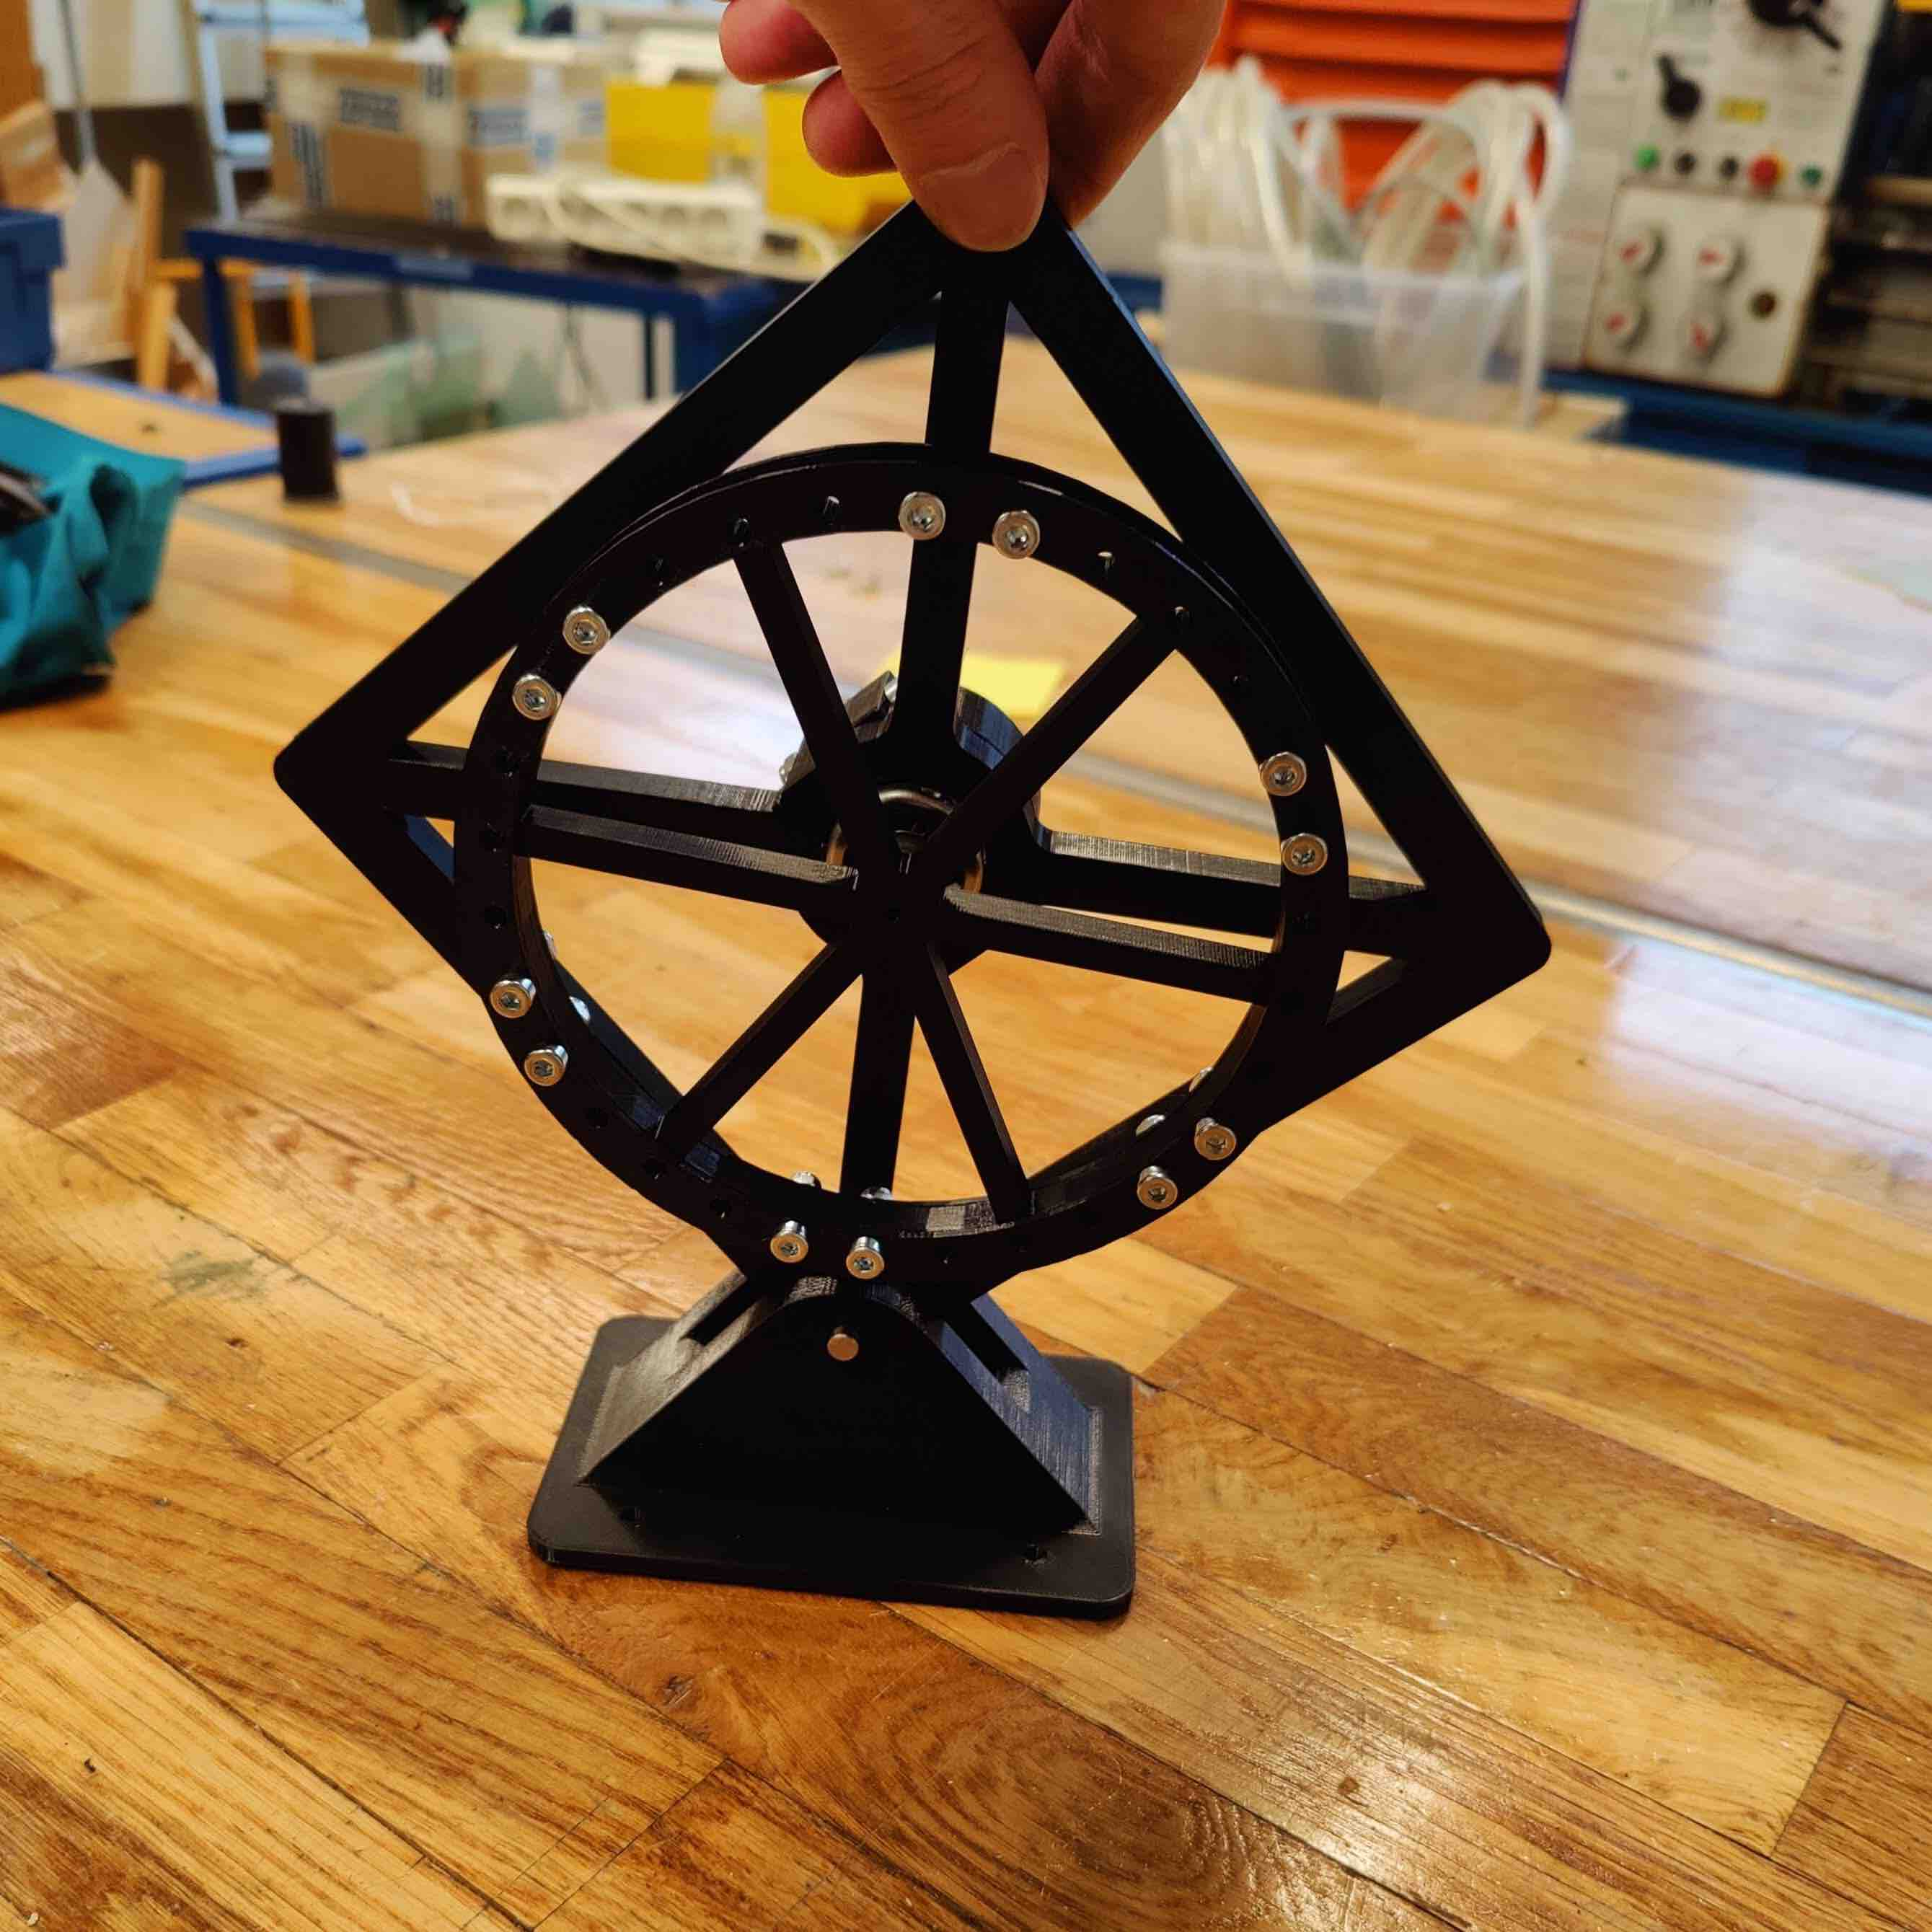
\includegraphics[width=0.6\linewidth]{figures/SingleAxisV1.jpg}
    \caption{The first version of the single axis setup}
    \label{fig:SingleAxisV1}
\end{figure}

\begin{figure}
    \centering
    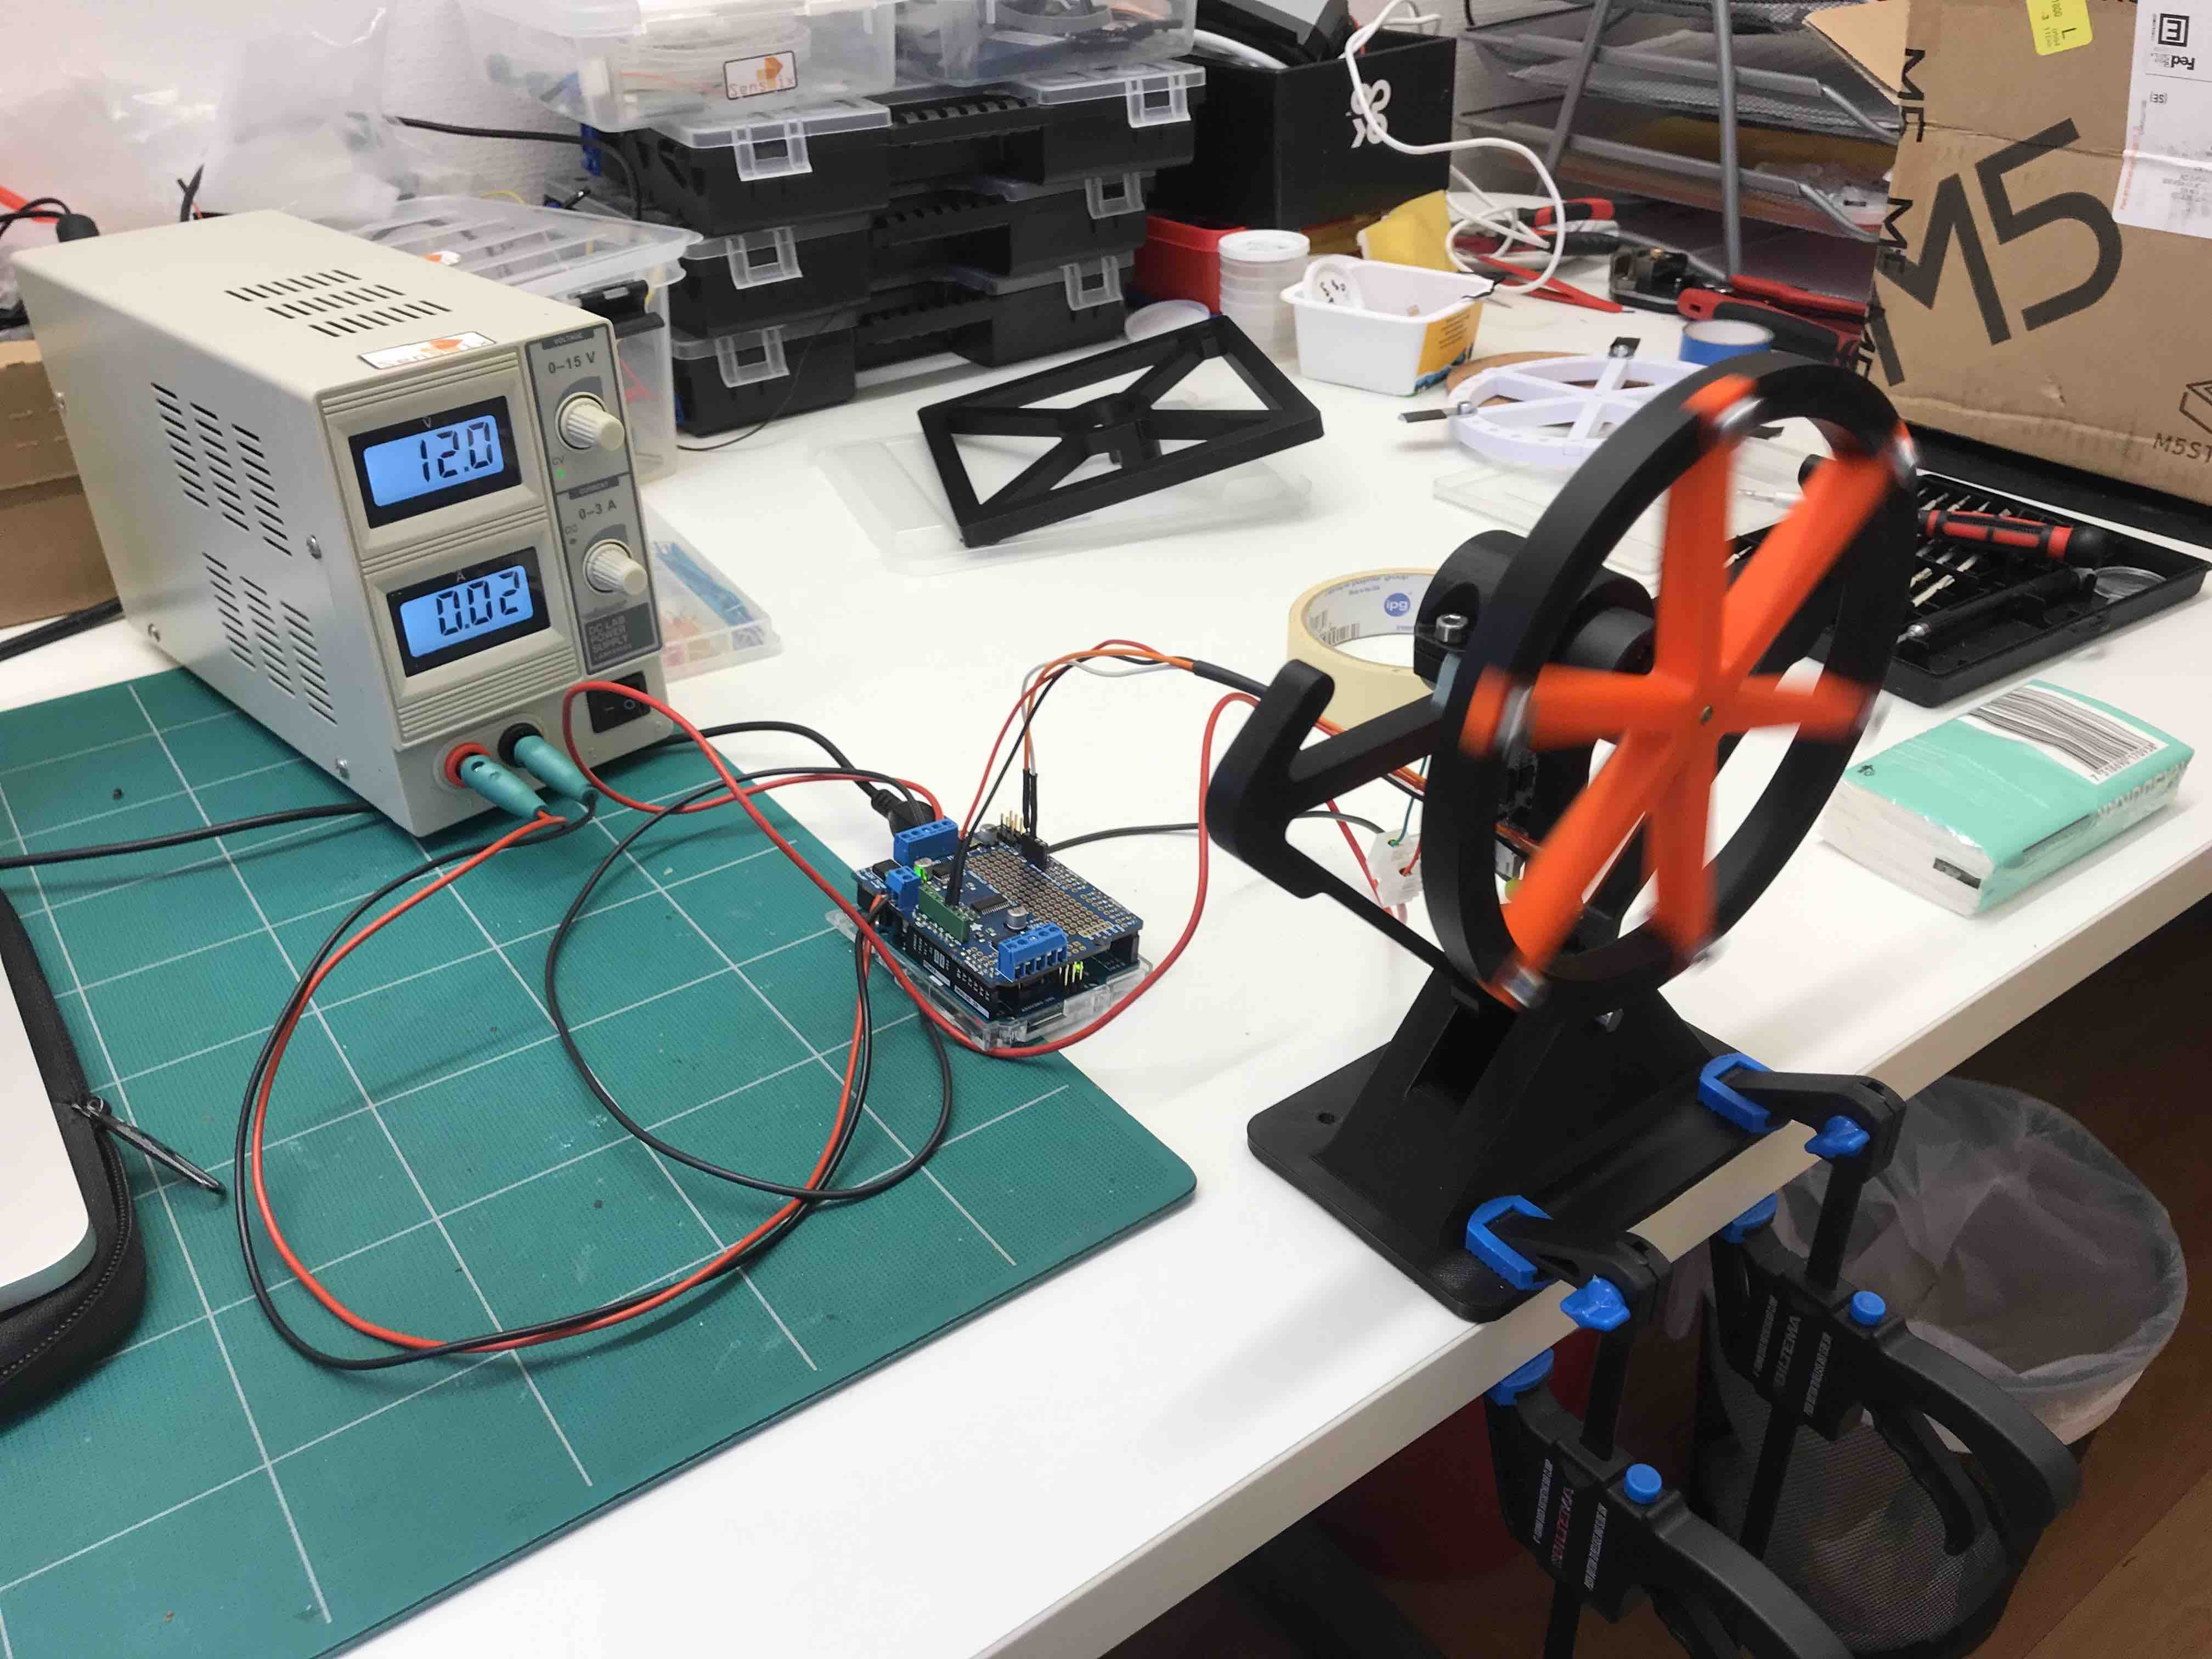
\includegraphics[width=.8\linewidth]{figures/SingleAxisV2Front.jpg}
    \caption{The second version of the single axis setup, with electrical components}
    \label{fig:SingleAxisV2}
\end{figure}

\subsection{The cube}
Designing the structure for the cube proved to be a lot more difficult and time consuming than expected. The intricate design demanded things to be decided based on assumptions, which later turned out to be incorrect. Some parts had to be redesigned multiple times. Some parts, e.g. four sides of the cube, were made identical to make the printing process less difficult. Other parts, engine mounts among them, were made symmetrical for the same reason. An advantage of having multiple identical parts is that if one part fails, it can potentially be replaced by another. While the replacement part is being printed, a side of the cube that is not critical when testing can be relocated into the critical position. The design of the cube can be seen in Figure~\ref{fig:cubediagram} with the parts named in Table~\ref{table:SystemComponents}.

%Här ska jonathans assembly bild in och referera till tabellen nedan.
\begin{figure}
    \centering
    \begin{subfigure}[h]{0.22\textwidth}
        \centering
        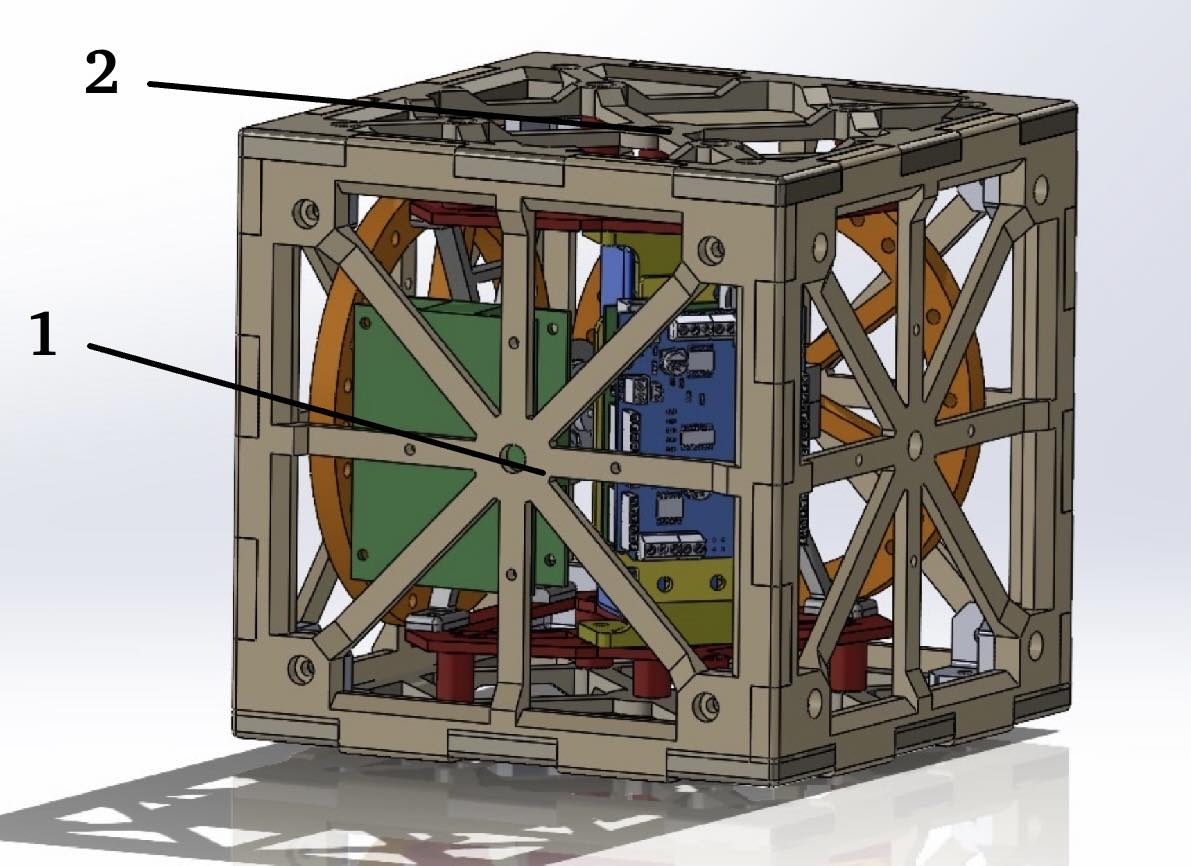
\includegraphics[width=\textwidth]{figures/Cube1.jpg}
    \end{subfigure}
    \begin{subfigure}[h]{0.22\textwidth}
        \centering
        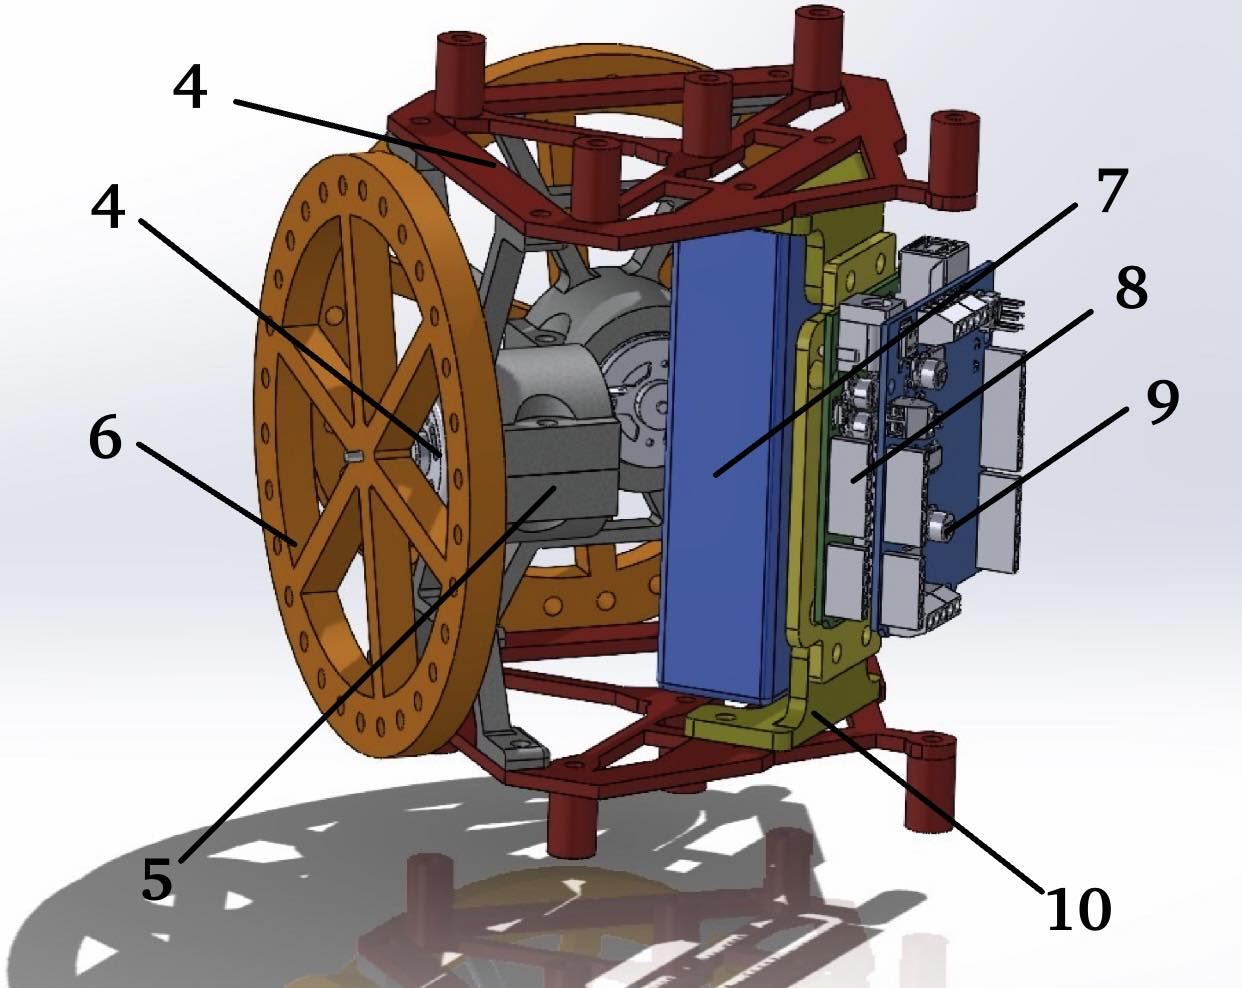
\includegraphics[width=\textwidth]{figures/cube2.jpg}
    \end{subfigure}
    \caption{The components in the system numbered.}
    \label{fig:cubediagram}
\end{figure}

\begin{table}
    \centering
    \begin{tabular}{cc}\toprule
     Component & Number \\\midrule
     Cube, side               & 1\\
     Cube, top and bottom     & 2\\
     Mounting plate           & 3\\
     DC motor                 & 4\\
     Motor holder             & 5\\
     Reaction wheel           & 6\\
     Battery                  & 7\\
     Arduino                  & 8\\
     Arduino Shield           & 9\\
     Electronics holder       & 10\\\bottomrule
    \end{tabular}
    \caption{The components in the system.}
    \label{table:SystemComponents}
\end{table}\label{sec:setup}

\section{System dynamics}
For both the cube and the single axis setup, the system dynamics can be analyzed in one plane only, provided the reaction wheel is parallel to that plane. In that case, the system is effectively an inverted pendulum constrained to one axis around a pivot point. When doing the mathematical analysis, we focused on the single axis setup as in Figure~\ref{fig:cubli_planar_diagram},

\begin{figure}[H]
    \centering
    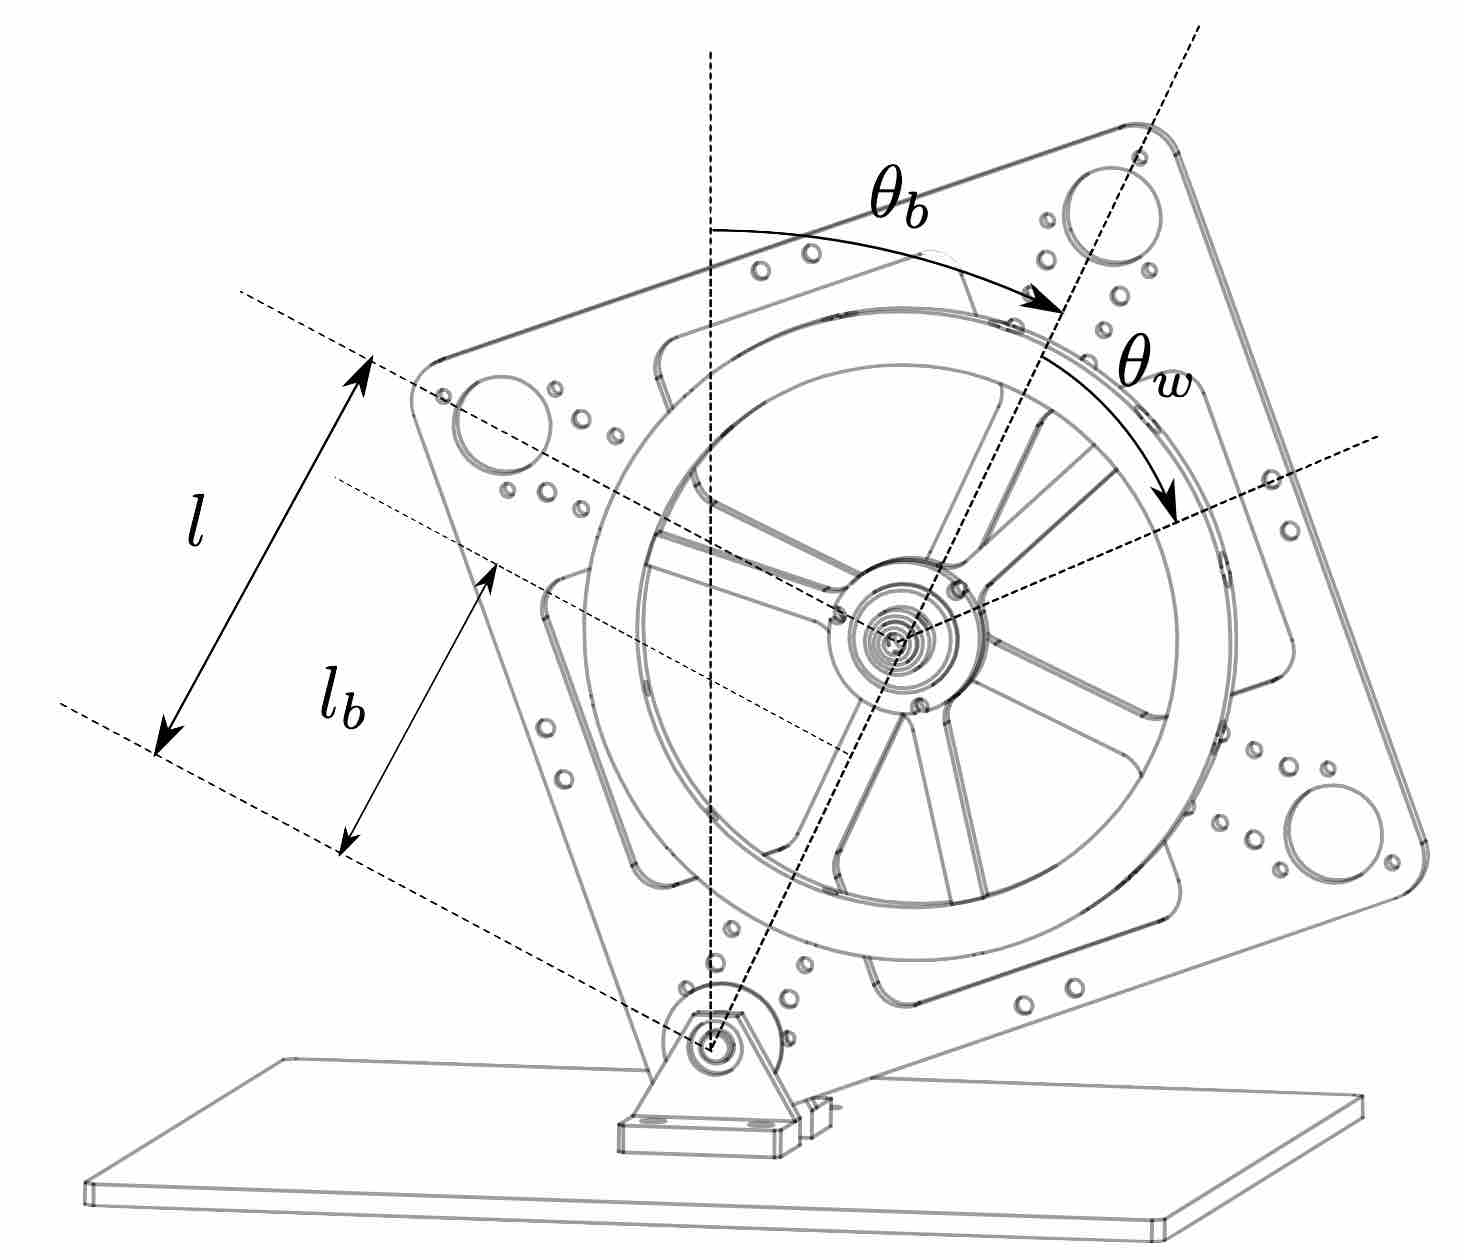
\includegraphics[width=.8\linewidth]{figures/Planar-diagram.jpg}
    \caption{Diagram of single axis setup from \cite{cubli-planar}.}
    \label{fig:cubli_planar_diagram}
\end{figure}

\noindent
where $\theta_b$ is the tilt angle of the pendulum body and $\theta_w$ is the angle of the wheel with respect to the body. The distance between the motor and the pivot point $O$ is denoted by $l$ whereas $l_b$ is the distance between the pendulum body's center of mass and $O$. Due to the symmetry of our prototype we assumed that $l = l_b$. We also assumed zero friction in the pivot point due to the use of a ball bearing. With these assumptions, we can modify the system of equations from \cite{cubli-planar} to get

\begin{equation}\label{eq:system}
    \begin{gathered}
        \ddot\theta_b = \frac{(m_b + m_w)gl\sin\theta_b - T_m +C_w\dot\theta_w}{I_b + m_wl^2}, \\
        \ddot\theta_w = \frac{(I_b + I_w + m_wl^2) \left( T_m - C_w\dot\theta_w \right)}{I_w(I_b + m_wl^2)} \\- \frac{(m_b + m_w)gl\sin\theta_b}{I_b + m_wl^2},
    \end{gathered}
\end{equation}

\noindent
where $m_b$ is the mass of the structure and the motor, $m_w$ is the mass of the reaction wheel, $T_m$ is the motor torque, $C_w$ is the dynamic friction coefficient of the wheel. $I_w$, $I_b$ are the moments of inertia of the wheel around its rotational axis and the pendulum body around $O$ respectively.

\subsection{Motor dynamics}
The motors used were initially simple brushed DC motors whose relation between torque $T_m$ and current $i$ drawn by the motor can be described as

\begin{equation}
    T_m = K_mi,
\end{equation}

\noindent
where $K_m$ is the torque constant. We can hence describe the acceleration of the reaction wheel as

\begin{equation}\label{eq:motor}
    \ddot\theta_w = \frac{K_m i - C_w\dot\theta_w}{I_w}.
\end{equation}

\subsection{State-space model}
We can now combine \eqref{eq:system} and \eqref{eq:motor} to get a full model that accounts for the current $i$. By using the approximation of small angles, $\sin\theta \approx \theta$, the system of equations becomes linear. The state variables are chosen as $\mathbf{x} = [\theta_b \ \dot\theta_b \ \dot\theta_w]^T$. Linearizing around $[0 \ 0 \ 0]^T$ gives

\begin{equation}\label{eq:state-space}  
    \begin{gathered}
        \dot{\mathbf{x}} = A\mathbf{x} + Bu, \\
        \mathbf{y} = C\mathbf{x},
    \end{gathered}
\end{equation}

\noindent
where

\begin{equation}\label{eq:ss-matrices}
    \begin{gathered}
        A =
        \begin{bmatrix}
            0 & 1 & 0 \\
            \frac{(m_b+m_w)gl}{I_b+m_wl^2} & 0 & \frac{C_w}{I_b+m_wl^2} \\
            -\frac{(m_b+m_w)gl}{I_b+m_wl^2} & 0 & -\frac{C_w(I_b+I_w+m_wl^2)}{I_w(I_b+m_wl^2)}
        \end{bmatrix}
        , \\
        B =
        \begin{bmatrix}
            0 \\
            -\frac{K_m}{I_b + m_wl^2} \\
            \frac{K_m(I_b+I_w+m_wl^2)}{I_w(I_b+m_wl^2)}
        \end{bmatrix}
        \text{ and } C =
        \begin{bmatrix}
            1 & 0 & 0 \\
            0 & 1 & 0 
        \end{bmatrix},
    \end{gathered}
\end{equation}

\noindent
where the control signal $u$ is the current $i$ and the output signal $\mathbf{y}$ is both $\theta_b$ and $\dot\theta_b$. The goal is to control only $\theta_b$ and stabilize it around 0, but the angular velocity $\dot\theta_b$ will also be directly readable from sensor data.
\\\\
The state-space model was then discretized using zero-order hold to get the discrete-time model

\begin{equation}\label{eq:ss-disc}
    \begin{gathered}
        \mathbf{x}_{k+1} = A_d\mathbf{x}_k + B_du_k,\\
        \mathbf{y}_k = C\mathbf{x}_k,
    \end{gathered}
\end{equation}

\noindent
where $A_d$ and $B_d$ are the discrete-time counterparts to $A$ and $B$.

\subsection{Parameter identification}
To simulate the state-space model, the physical parameters had to be identified. $I_b$ was calculated with

\begin{equation}\label{eq:Ib}
    I_{b} = \frac{s_{f}^2}{6}m_{f} + \frac{r_{m}^2}{2}m_{m} + (m_{f} + m_{m})l^2,
\end{equation}

\noindent
where $s_{f}$ is the side length of the frame, $r_{m}$ is the radius of the motor, $m_{f}$ is the mass of the frame and $m_{m}$ is the mass of the motor. $I_w$ was calculated with

\begin{equation}\label{eq:Iw}
    I_{w} = \frac{1}{2}m_{w}(r_{\text{outer}}+r_{\text{inner}})^2
\end{equation}

\noindent
where $r_{\text{outer}}$ is the radius of the wheel and $r_{\text{inner}}$ is the radius to the inner edge of the wheel. The maximum torque of the motor can be found in \cite{motor-datasheet}. The torque constant $K_{m}$ can also be calculated from the data sheet, using the equation

\begin{equation}\label{eq:Km}
    K_{m} = \frac{T_{2} - T_{1}}{i_{2} - i_{1}},
\end{equation}

\noindent
where the torques $T_1, T_2$ and currents $i_1, i_2$ were chosen at two different points.
\label{sec:dynamics}

\section{Controlling the process}
Two control strategies were considered, PID-control and an observer-based controller using LQG.

\subsection{PID-control}
The PID controller continuously reads the current output signal $\theta_b(t)$ and compares it to the reference signal $r(t)$ to calculate the current error $e(t) = r(t) - \theta_b(t)$. The control signal $u(t)$ is then decided according to

\begin{equation}\label{eq:PIDcont}
    u(t) = K_P e(t) + K_I \int_0^t e(\tau) \ d\tau + K_D \frac{d}{dt}e(t),
\end{equation}

\noindent
where the control parameters $K_P$, $K_I$ and $K_D$ are predetermined. Since the objective is to balance a pendulum, i.e., make $\theta_b=0$. The reference will therefore be set to $r=0$. Since the controller has to be discretized in the implementation the integral is replaced by a sum and the derivative by a difference quotient. If the output signal is read at time intervals of $\Delta t$ we get

\begin{equation}\label{eq:PIDdisc}
    \begin{gathered}
        u(t) = K_Pe(t) + K_I \sum_{k=0}^N [e(k\Delta t)\Delta t] + K_D \frac{e(t) - e(t-\Delta t)}{\Delta t}, \\
        t = N\Delta t,
    \end{gathered}
\end{equation}

\noindent
for the number of samples $N$. The sampling time $\Delta t$ can be baked into the parameters $K_I$ and $K_D$ leading to fewer calculations in the code implementation. For ease of reading we let 

\begin{equation}
    \begin{gathered}
        I(t) = \sum_{k=0}^N [e(k\Delta t)\Delta t], \\
        D(t) = \frac{e(t) - e(t-\Delta t)}{\Delta t}, \\
        t = N\Delta t.
    \end{gathered}
\end{equation}

\subsection{Additions to the PID controller}
The first addition is adjusting the reference signal based on the current error. If the reference is moved further away from the current output the error will be larger and the controller will have a stronger response. For an angle increment of $\Delta\theta$ the updated reference angle $r(t+\Delta t)$ will be

\begin{equation}\label{eq:ref-adjustment}
    r(t+\Delta t) =
    \begin{cases}
        r(t) + \Delta\theta, \ \ \ e(t) > 0. \\
        r(t) - \Delta\theta, \ \ \ e(t) < 0.
    \end{cases}
\end{equation}

\noindent
This will have the most significant impact on the integral part of the controller. The increment value should be relatively small, especially with a quick sample time, otherwise the controller may not be able to catch up. This can be beneficial if you want especially the integral part to grow quickly. We also introduce an integral saturation $I_{\text{max}}$, making the sum $I(t)$ capped to $\pm I_{\text{max}}$.
\\\\
Another addition to the PID controller was motor feedback. This was achieved by having the control signal feedback into itself. With a discretized controller this becomes quite simple by introducing a fourth control parameter, $K_C$, and adding the term $K_Cu(t-\Delta t)$ to equation \eqref{eq:PIDdisc}, giving

\begin{equation}\label{eq:PIDCdisc}
    u(t) = K_P e(t) + K_I I(t) + K_D D(t) + K_C u(t-\Delta t).
\end{equation}

\subsection{LQG control}
First, we introduce independent disturbance and noise processes $\mathbf{w}_k$ and $\mathbf{v
}_k$ into the discrete-time system from \eqref{eq:ss-disc} to get

\begin{equation}
    \begin{gathered}
        \mathbf{x}_{k+1} = A_d\mathbf{x}_k + B_du_k + \mathbf{w}_k, \\
        \mathbf{y}_k = C\mathbf{x}_k + \mathbf{v}_k.
    \end{gathered}
\end{equation}

\noindent
Let both processes be white Gaussian noise with covariance matrices $V$ and $W$ respectively. By introducing a Kalman filter and state feedback we form the control equations

\begin{equation}\label{eq:LQG}
    \begin{gathered}
        \hat{\mathbf{x}}_{k+1} = A_d\hat{\mathbf{x}}_k + B_du_k + L(\mathbf{y}_k - C\hat{\mathbf{x}}_k),\\
        u_k = K\hat{\mathbf{x}}_k,
    \end{gathered}
\end{equation}

\noindent
where $\hat{\mathbf{x}}_k$ is the estimated state vector. In order to use equation \eqref{eq:LQG}, both matrices $K$ and $L$ need to be determined. They were determined by solving the linear-quadratic-Gaussian (LQG) optimal control problem. The feedback gain $K$ is chosen such that it minimizes the cost function

\begin{equation}\label{eq:LQG-cost}
    J(u) = \sum_{k=1}^\infty \mathbf{x}_k^T Q \mathbf{x}_k + u_k^T R u_k,
\end{equation}

\noindent
for some weight matrices $Q$ and $R$. Both the feedback gain $K$ and the Kalman gain $L$ can be obtained by solving their respective algebraic Riccati equations. This was done in Matlab using the commands \texttt{dlqr} and \texttt{dlqe}, which determines the $K$ and $L$ matrices respectively. For \texttt{dlqr}, the weight matrices had to be chosen, which was done by experimenting with different penalties. For \texttt{dlqe}, the covariance matrix for the measurement noise could be estimated using measured data. Estimating the covariance matrix for the noise affecting the states is difficult, and therefore an identity matrix is used instead.

\subsection{Motor limitations}
Most of the components used were off-the-shelf components, that were available at the university. This was a limiting factor, especially in terms of motors. A weak motor that provides low torque, puts a restriction on the maximum recovery angle. By analyzing the system statically at some tilt angle $\alpha$, we can calculate the motor torque necessary to cancel out the torque $T_O$ in the pivot point due to the gravitational force on the system. The torque $T_O$ can be calculated as

\begin{equation}\label{eq:tau}
    T_O = (m_b^*+m_w)gl \sin \alpha,
\end{equation}

\noindent
where $m_b^*$ is the mass of the pendulum body and the motor being considered. This equation was used to estimate motor requirements depending on the mass of the motor and desired recovery angles. The torque $T_O$ can be seen as the bare minimum to recover from $\alpha$. In practice, much higher torque is required if the pendulum is to also accelerate towards the equilibrium. Note also that the pendulum will not be still when at this angle $\alpha$. It will have fallen there and thus have a non-zero angular velocity, requiring an even higher torque.

\subsection{Sampling limitations}
Apart from torque generation in the motors, the sampling time is also an important factor. In these types of unstable (open loop) systems a quick sampling rate is of critical importance in order to recover from disturbances before it is too late. Although a fast sampling rate is desired, it is limited by the hardware. The most limiting factor for the sampling time was the IMU, which outputs data at 100 Hz\cite{IMU-datasheet} i.e. a sample time of 10 ms.\label{sec:control}

\section{Results}
\subsection{Selecting the new motor}
Out of the available off-the-shelf motors the L1491210\cite{motor-datasheet} from Micro Motors was selected. According to \eqref{eq:tau}, it should momentarily hold a tilt angle of $4\degree$, which was more than twice as powerful as the first motor used.

\subsection{Physical parameters}
The physical parameters were identified for the single axis setup. These values were used for the simulations and can be found in Table~\ref{table:MeasuredValues}.

\begin{table}[h]
    \centering
    \begin{tabular}{cc}\toprule
            Parameter  & Value \\\midrule
            $I_{b}$      & $2.1 \cdot 10^{-3} \text{ kg} \cdot \text{m}^2$ \\
            $I_{w}$      & $6.4 \cdot 10^{-3} \text{ kg} \cdot \text{m}^2$ \\
            $m_{b}$      & 0.170 kg \\
            $m_{w}$      & 0.076 kg \\
            $l$            & 0.093 m \\
            $K_{m}$      & 0.5 Nm/A \\
            $T_{\text{max}}$    & 0.015 Nm \\\bottomrule
    \end{tabular}
    \caption{Parameters and their measured values.}
    \label{table:MeasuredValues}
\end{table}

\noindent
The only parameter that was not identified was the friction coefficient, $C_{w}$. Instead, the same value as the one in \cite{cubli-planar} was used, $C_{w} = 5 \cdot 10^{-5} \text{ kg} \cdot \text{m}^2 \cdot \text{s}^{-1}$.

\subsection{Measurements from the IMU}
The structure was tilted slowly from side to side while the angle was measured at 10 ms intervals. The results can be seen in Figure~\ref{fig:imu_angle}.

\begin{figure}[H]
    \centering
    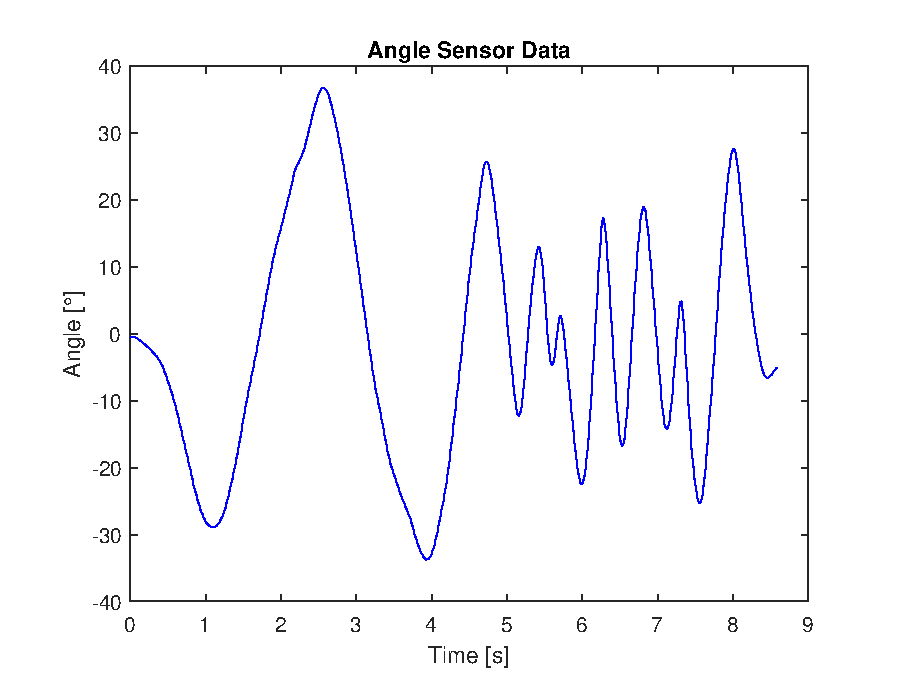
\includegraphics[width=.9\linewidth]{figures/plot_angle.eps}
    \caption{Angle measurements from the IMU.}
    \label{fig:imu_angle}
\end{figure}

\noindent
The structure was then laid still while the angular velocity from the gyrometer was measured at 10 ms intervals. The results can be seen in Figure~\ref{fig:imu_gyro}.

\begin{figure}[H]
    \centering
    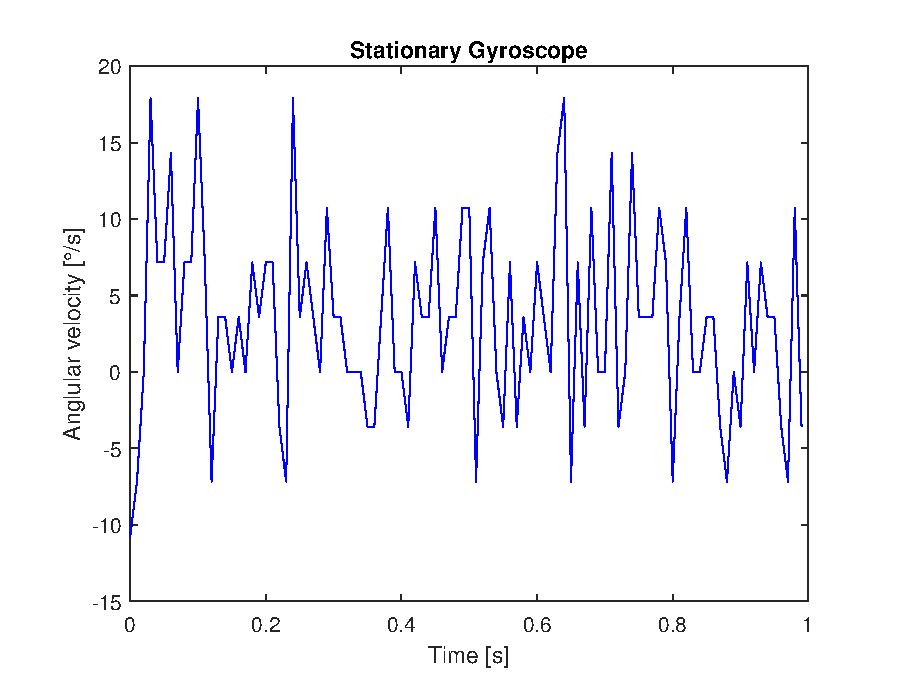
\includegraphics[width=.9\linewidth]{figures/plot_stationary.eps}
    \caption{Angular velocity measurements from the IMU.}
    \label{fig:imu_gyro}
\end{figure}

\subsection{Simulations}
The model in \eqref{eq:state-space} and \eqref{eq:ss-matrices} was simulated using both a PID controller and a LQG controller. The simulation results can be seen in Figure~\ref{fig:PIDGraph} and Figure~\ref{fig:LQGGraph}. For both simulations, a sample time of 15 ms and a pulse disturbance of $0.5\degree$ was used.
\\\\
The parameter settings for the discrete PID controller can be seen in Table~\ref{table:PIDParameters}.

\begin{table}[H]
    \centering
    \begin{tabular}{cc}\toprule
     Parameter  & Value \\\midrule
     $K_{P}$      & 3\\
     $K_{I}$      & 1\\
     $K_{D}$      & 0.3\\\bottomrule
    \end{tabular}
    \caption{The chosen PID parameters.}
    \label{table:PIDParameters}
\end{table}

\noindent
The optimal gain matrices $K$ and $L$ were calculated as

\begin{equation}
    \begin{gathered}
        K =
        \begin{bmatrix}
            6.0497 & 0.7365 & 0.0611
        \end{bmatrix}
        ,\\
        L = 
        \begin{bmatrix}
            1       & 0\\
            14.0934 & 0.0825\\
            0.8845  & 0.0048\\
        \end{bmatrix}
        .
    \end{gathered}
\end{equation}

\begin{figure}[h]
    \centering
    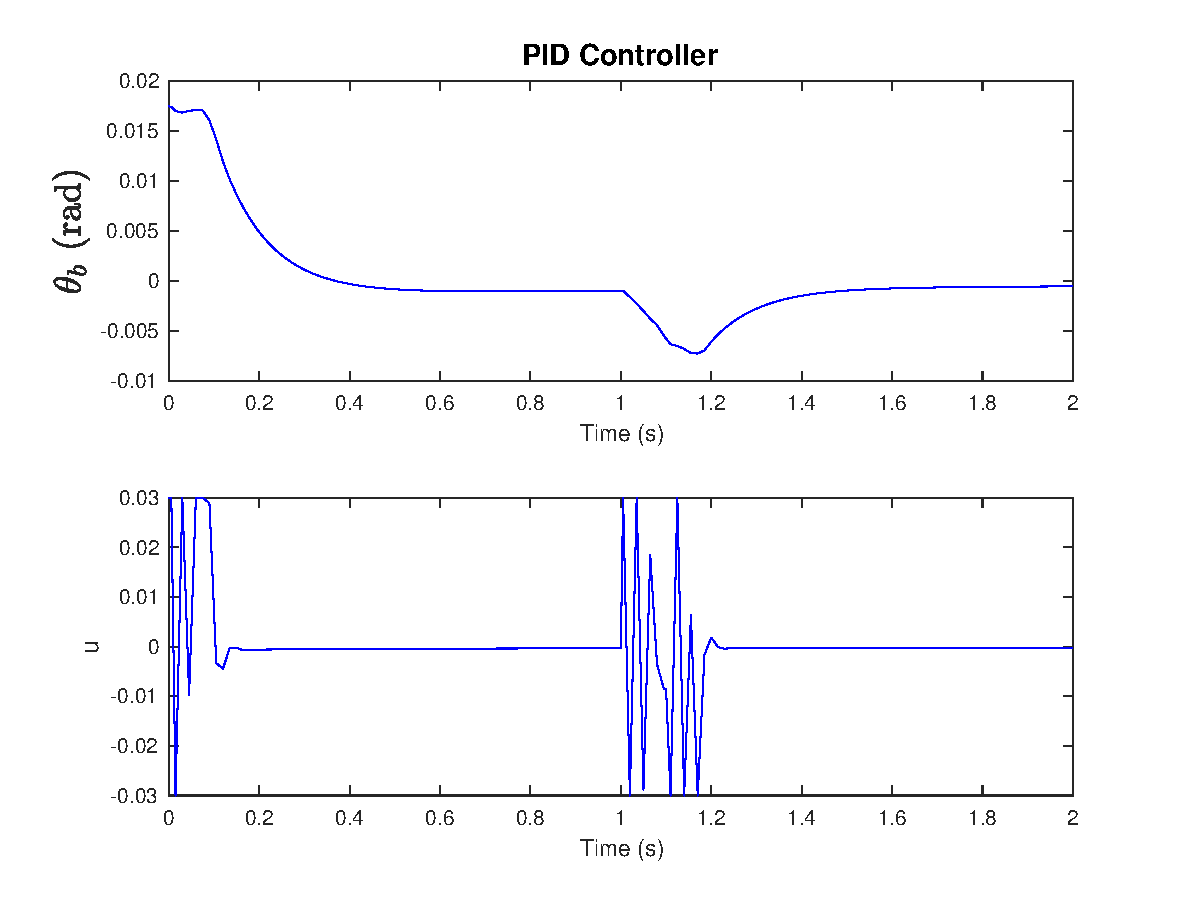
\includegraphics[width=\linewidth]{figures/PID.eps}
    \caption{Simulation of the single axis setup with a disturbance, using the PID controller.}
    \label{fig:PIDGraph}
\end{figure}

\begin{figure}[h]
    \centering
    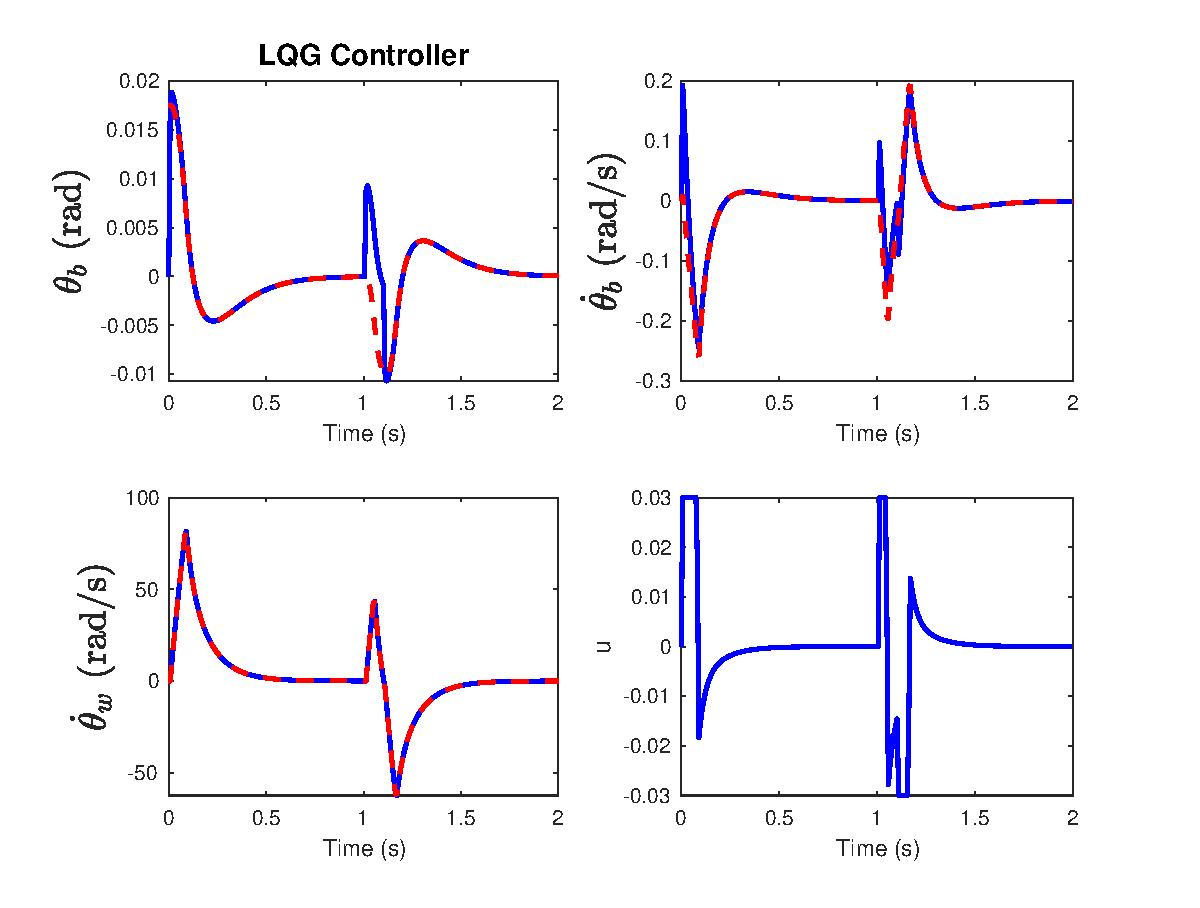
\includegraphics[width=\linewidth]{figures/LQG.eps}
    \caption{Simulation of the single axis setup with a disturbance, using the LQG controller. The blue line represents the estimated values and the red dashed line represents the values calculated from the state-space model.}
    \label{fig:LQGGraph}
\end{figure}

\noindent
While experimenting with different parameter settings for the simulation, we observed that some had a larger effect on the system than others. By changing the parameters in the PID simulation, with different factors, the parameters importance could be observed. The observation was based on how high, or low, of a factor a parameter could handle, before the system achieved instability. Sampling time, maximum torque and length to center of mass had the largest effect. This was followed by the mass of the frame and the radius of the wheel. In contrast, the system was still stable with a high friction coefficient and a low mass of the wheel. This qualitative observation is summarized in Table~\ref{table:ParamSig}.

\begin{table}[H]
    \centering
    \begin{tabular}{ccc}\toprule
            Parameter  & Factor & Importance \\\midrule
            $\Delta t$        & 1.2         & Very high\\
            $T_{\text{max}}$  & $2.7^{-1}$  & High\\
            $l$               & 2.8         & High\\
            $m_b$             & 4.5         & Medium\\
            $r_{w}$           & $4.5^{-1}$  & Medium\\
            $m_{w}$           & $< 20^{-1}$ & Low\\
            $C_{w}$           &  40         & Low\\\bottomrule
    \end{tabular}
    \caption{Parameters and their observed importance.}
    \label{table:ParamSig}
\end{table}

\subsection{The physical setup}
The discretized controller from \eqref{eq:PIDdisc} was implemented with a sample time of 10 ms with the original DC motors given to us. The motor was eventually swapped out to the new one\cite{motor-datasheet}. After this, testing could begin again. This time the motor feedback from \eqref{eq:PIDCdisc} was also implemented. Experimenting with PD-control and positive values of $K_C$ seemed promising but balancing still proved difficult. In a last ditch effort a new design for the pendulum body was made. The improved structure can be seen in Figure~\ref{fig:SingleAxisV2}.
\\\\
After some inspiration from\cite{LEGO-video} the controller now made use of integral action with a positive $K_I$ as well as reference adjustment according to \eqref{eq:ref-adjustment}. $K_C$ was now chosen to be negative and relatively small. The idea was to slow down the wheel over time when balancing. After some tuning stable balancing was finally achieved with the following control parameters:

\begin{equation}
    \begin{gathered}
        K_P = 50, \ \ K_I = 150, \ \ K_D = 2.5, \ \ K_C=-0.2, \\
        I_{\text{max}} = 127, \ \ \Delta \theta = 0.004.
    \end{gathered}
\end{equation}

\noindent
Note that the control signal ranges between $\pm255$ (where 255 is simply the max speed of the motor) and the output signal is measured in degrees. The parameter $\Delta \theta$ is also in degrees. In the code implementation, $\Delta t$ was also baked into the constants to reduce the amount of calculations. In Figure~\ref{fig:physical-balance} we can see roughly 15 seconds of balance using the control parameters above. The sensor readings shown are spaced 50 ms apart, but the controller still acted at the usual 10 ms intervals.

\begin{figure}[H]
    \centering
    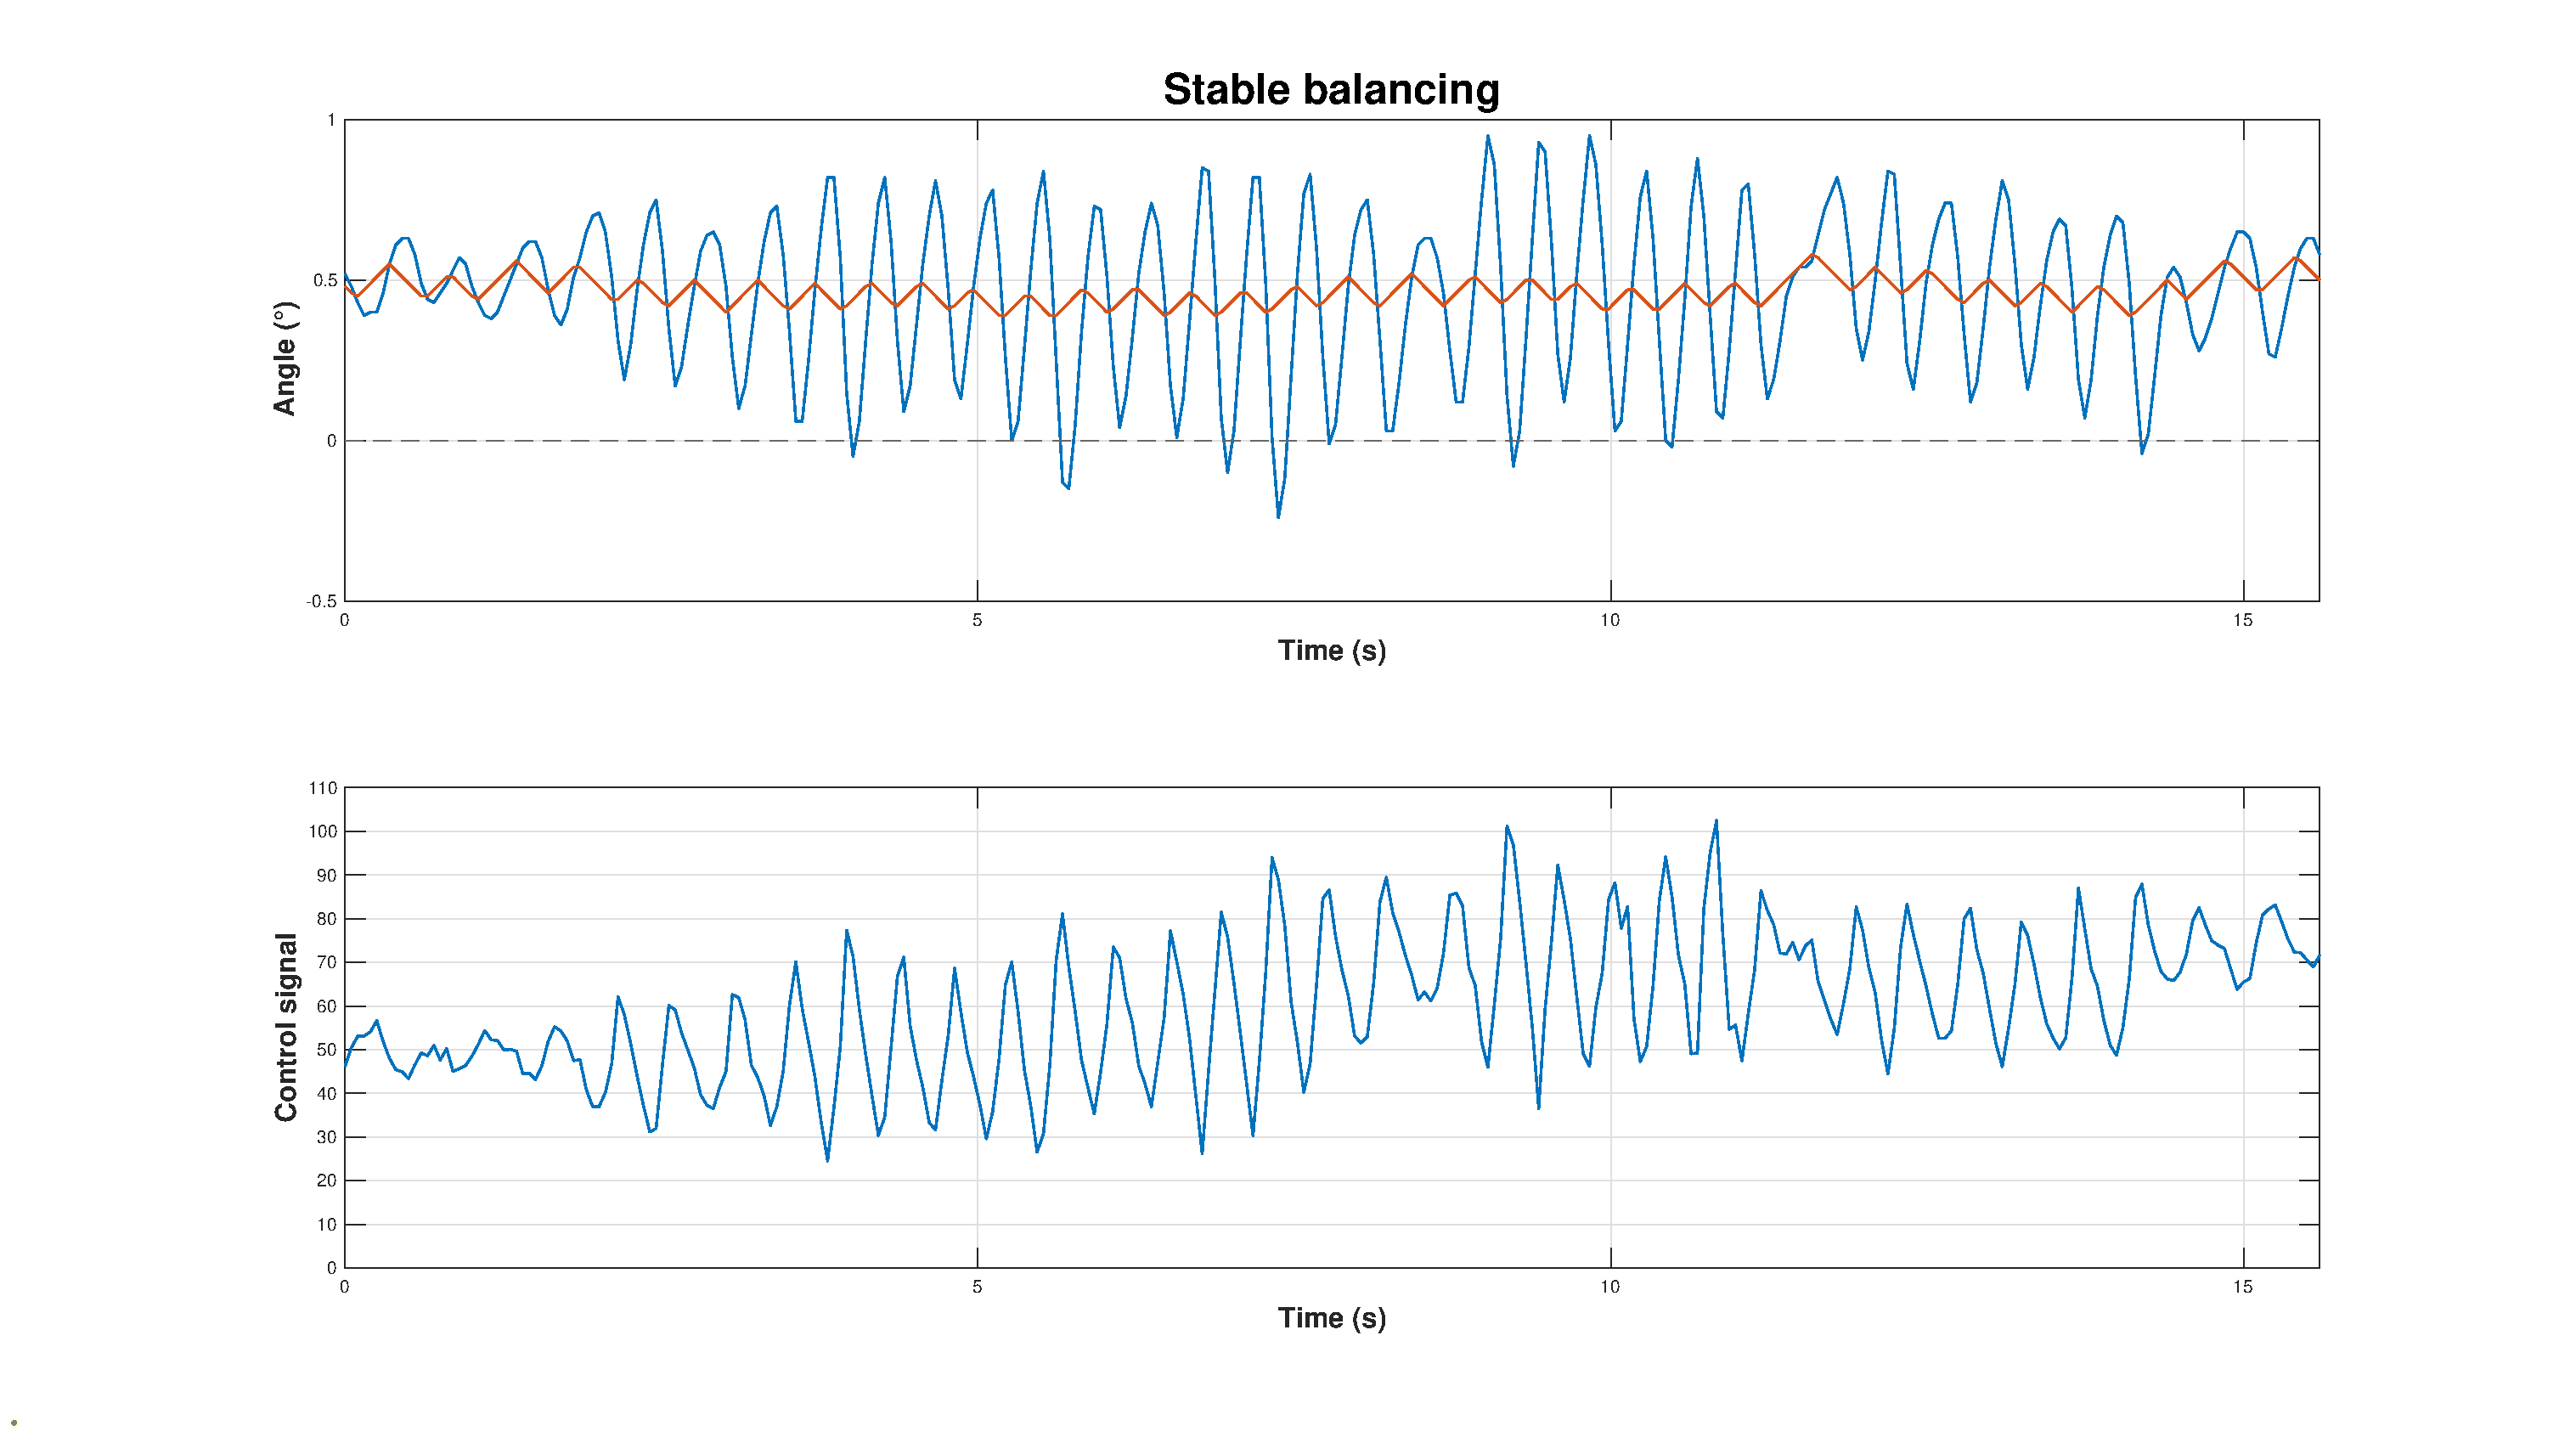
\includegraphics[width=1.2\linewidth, center]{figures/balance_with_u.eps}
    \caption{Top graph: the measured angle $\theta_b$ is in blue and $r$ is in orange. Bottom graph is the control signal.}
    \label{fig:physical-balance}
\end{figure}

\noindent
There are some key takeaways from this graph. Firstly, The structure is not balancing around $0\degree$. Instead, the reference is oscillating slightly around $0.46\degree$. The standard deviation in error over this period was $\sigma_e = 0.24\degree$. Secondly, the control signal is also oscillating around a positive, non-zero speed.
\\\\
Note that these 15 seconds were an excerpt from a longer period of balancing. In reality, the structure could balance for several minutes. The longest measured time balancing was just shy of 37 minutes. It could also handle small disturbances such as shaking the table and gently pushing the structure.

\subsection{The cube}
The physical model can be seen in Figure~\ref{fig:AssembledCube}. The printed parts, structural screws and nuts had a total mass of 587 grams. The scale that was used had an upper limit of 1 kg, which the cube exceeded with the rest of the internal components assembled.

\begin{figure}[H]
    \centering
    \begin{subfigure}[h]{0.2\textwidth}
        \centering
        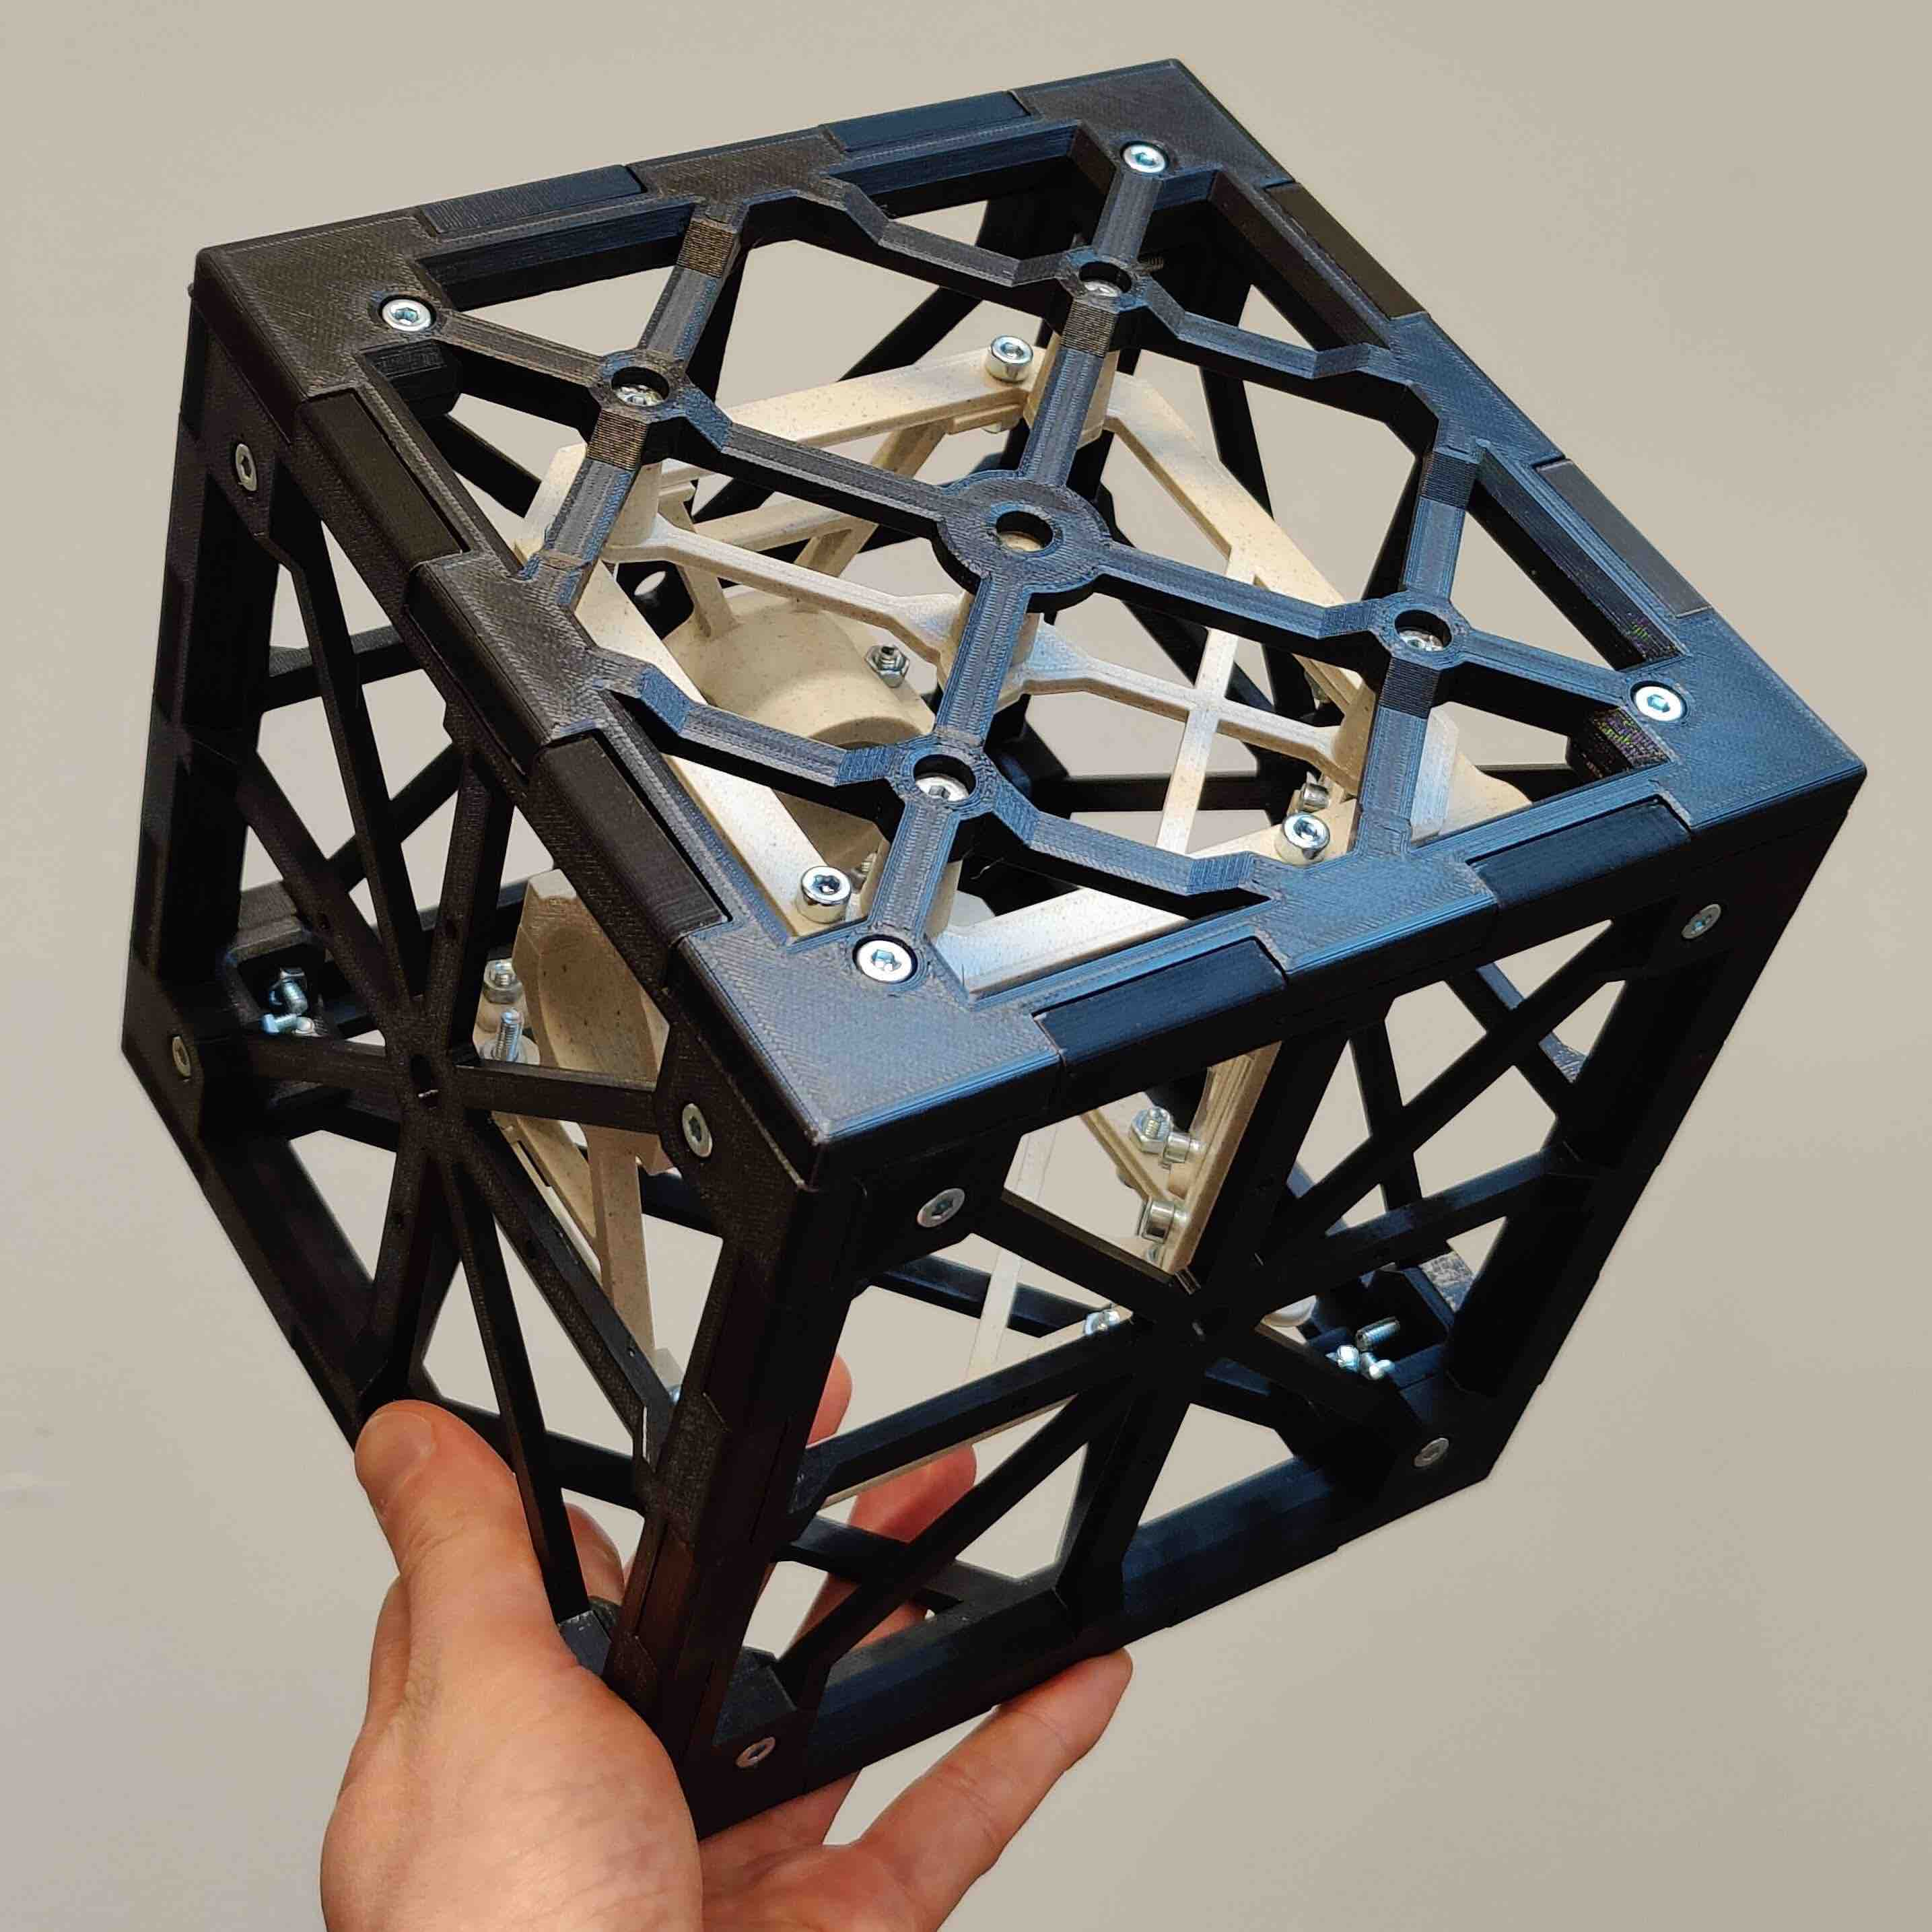
\includegraphics[width=\textwidth]{figures/CubeNoComponents.jpg}
        %\caption{Without electrical components}
        \label{fig:cubeNoComp}
    \end{subfigure}
    \begin{subfigure}[h]{0.2\textwidth}
        \centering
        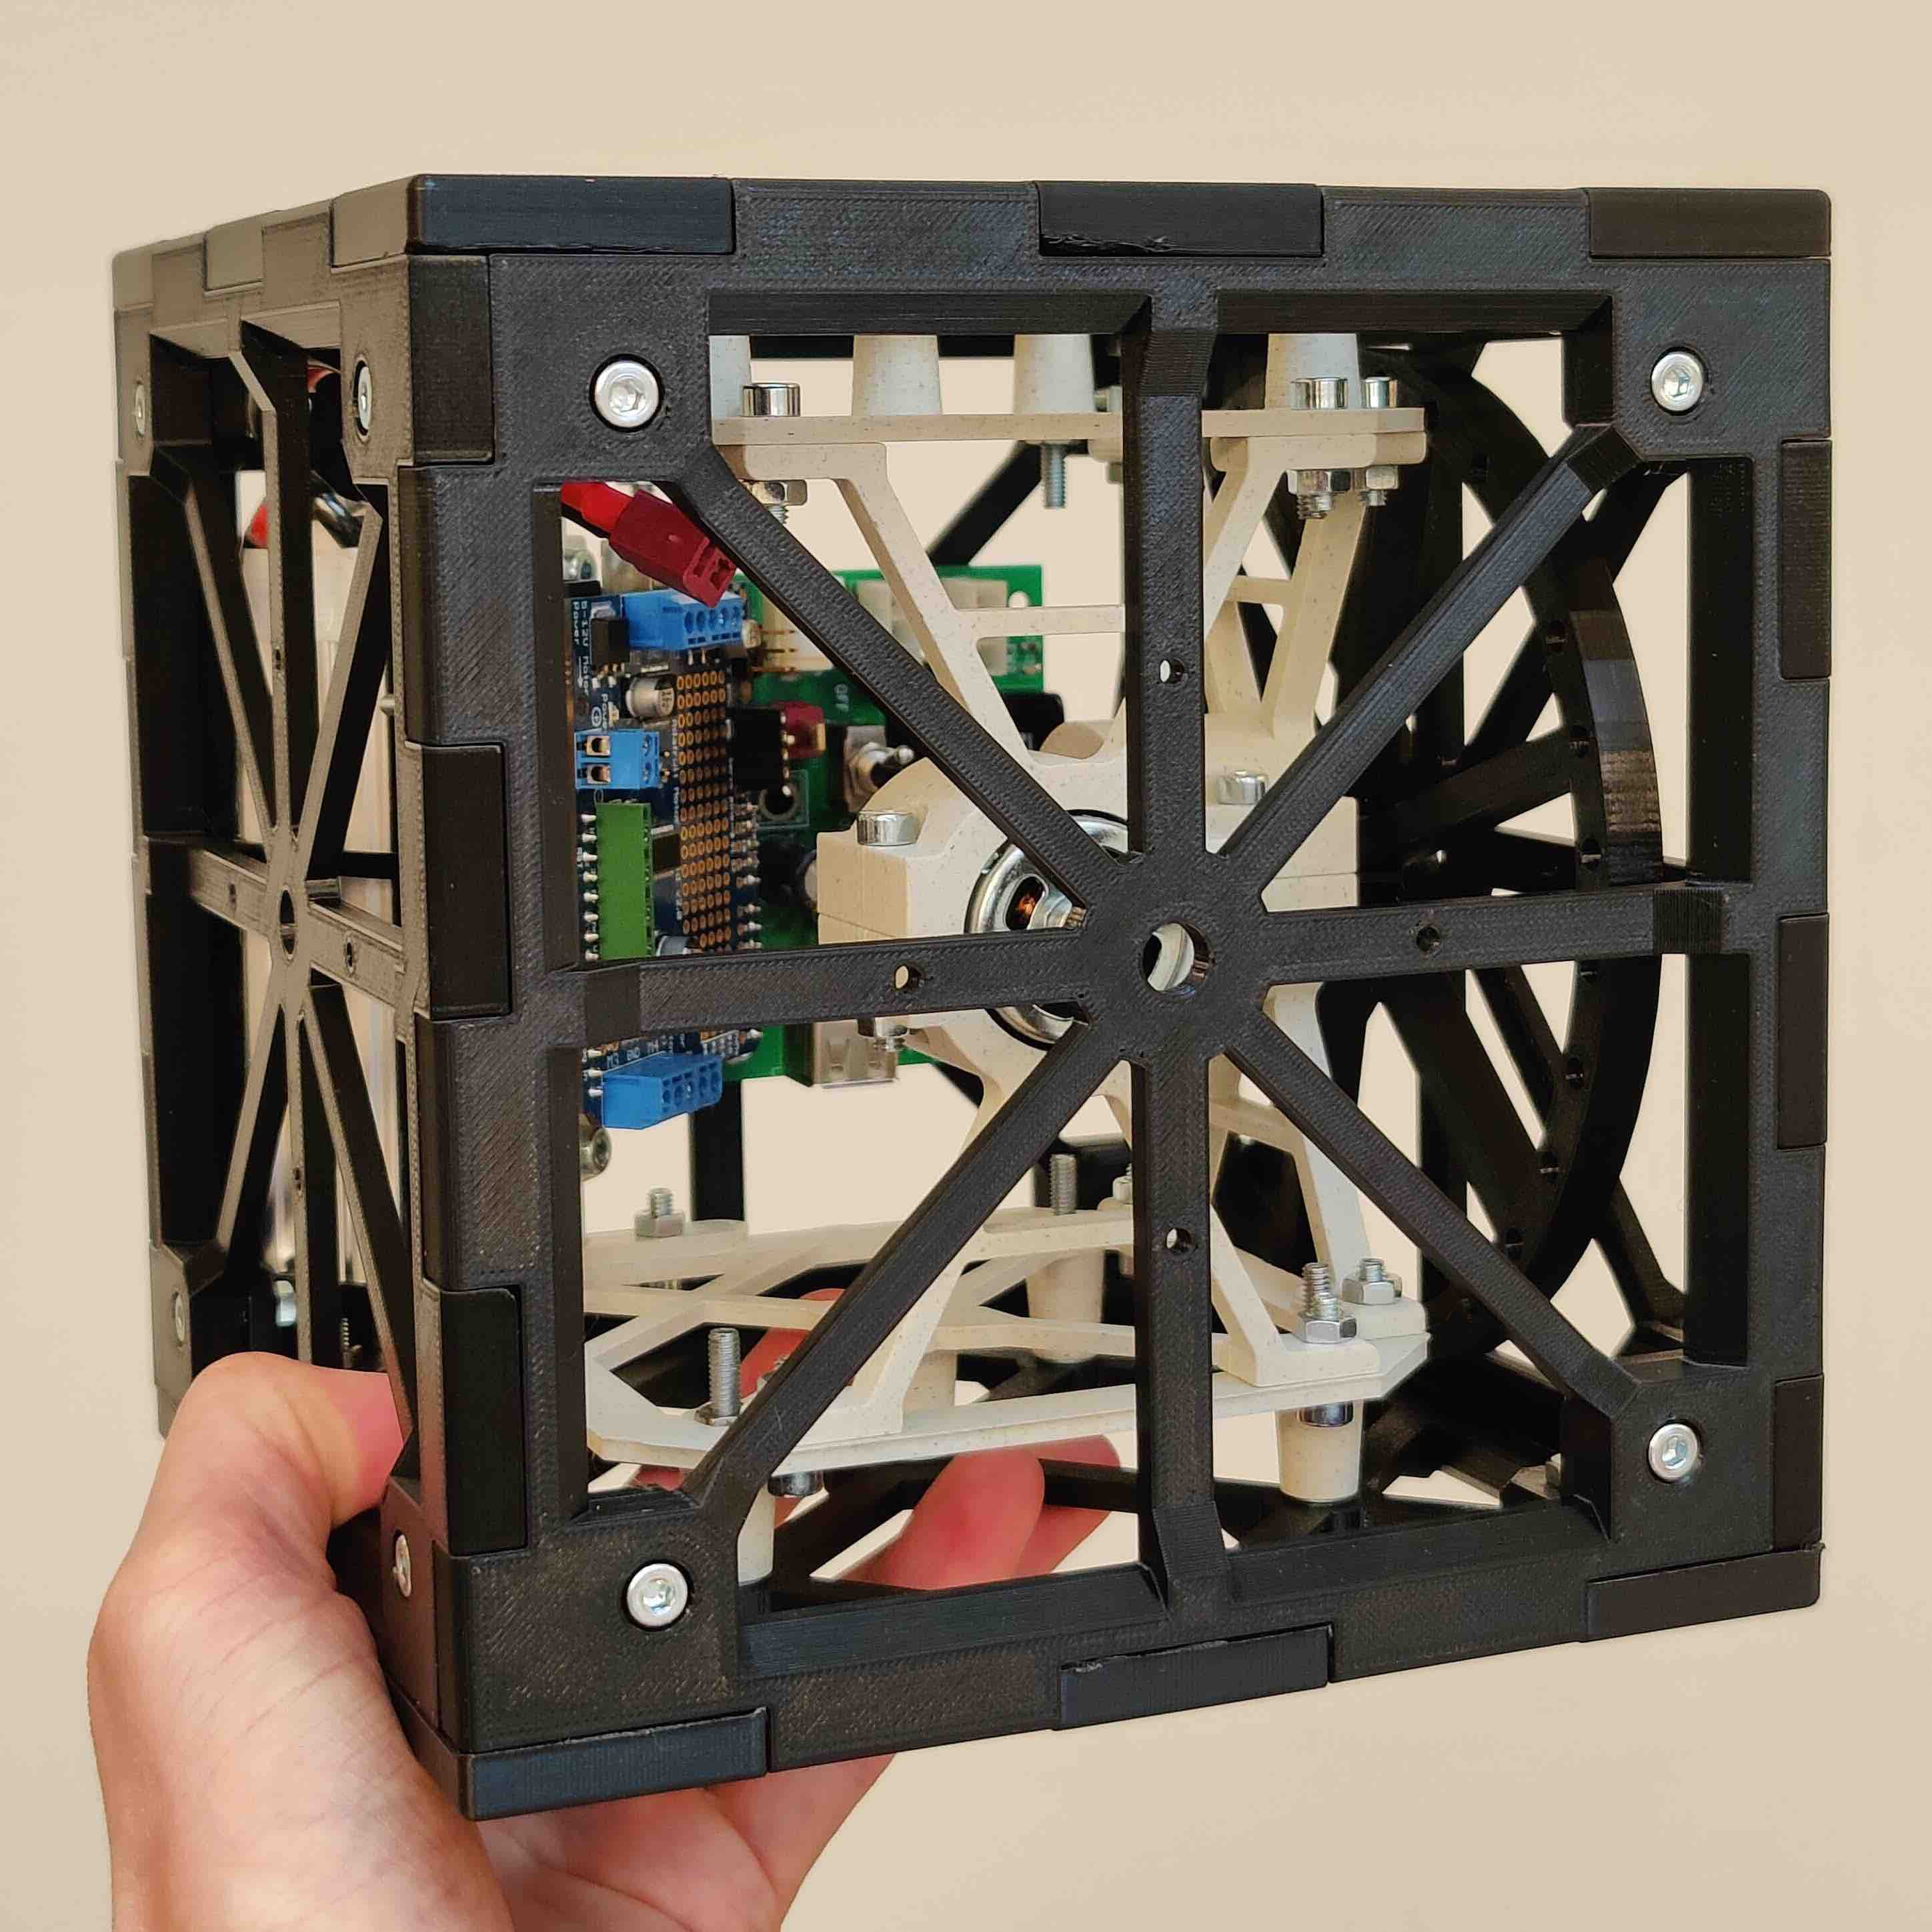
\includegraphics[width=\textwidth]{figures/CubeWithComponents.jpg}
        %\caption{With electrical components}
        \label{fig:cubeWith}
    \end{subfigure}
    \caption{The printed cube with and without components}
    \label{fig:AssembledCube}
\end{figure}
\label{sec:results}

\section{Discussion}
Our supervisor said during a meeting that "There are two ways of solving a control problem. Either, one designs the system and actively chooses which components are to be used, or one is given a complete system and has to do a lot more work on control modelling and algorithms."

\subsection{Limitations in the simulation}
There were a number of limitations in the simulation that has to be addressed. First of all, the simulation uses the linearized model in \eqref{eq:state-space}. This does not completely represent the reality of the dynamics of the single axis setup. However, since the working range of the angle of the system is only a couple of degrees, it was reasonable to use the linearized model. Second of all, many of the parameters used in the model were approximated. The moments of inertia were all derived using standard formulas and could have been more accurate. Another example is the friction coefficient, which was taken from \cite{cubli-planar}. Although there are a number of limitations to the simulation, the purpose of it was not to get a working controller that could be directly applied to the real model, but instead to see how a PID controller compares to a LQG controller, and which parameters are important.

\subsection{Interpreting the simulations}
As seen in Figures~\ref{fig:PIDGraph} and \ref{fig:LQGGraph}, both controllers could stabilize the system with the given set of parameters. They could also handle an impulse disturbance of $0.5\degree$. When comparing the two controllers, one instantly notes the smoother response of the LQG controller. However, the LQG is highly dependent on a good model of the system and to what extent our model and parameters are sufficient, will not be answered in this paper, since a LQG controller was not implemented in the real system. Both controllers in the simulation used a sampling time of 15 ms. This was done in order to insure that the sampling time was not impossible to meet.
\\\\
As mentioned in Table~\ref{table:ParamSig}, the most significant parameters were the sampling time, the maximum torque that the motor can generate and the length to center of mass from the pivot point. This is reasonable since a longer length to the center of mass will increase the torque required cancel the gravitational force. The motor torque is also important to counter the torque generated by the body itself. It is also reasonable that the sampling time is significant, since  even a small change in angle will have large effect on the necessary torque to counter the fall and the change in angle should be measured as fast as possible. Also, the mass of the frame and the radius of the wheel, seemed less important. This is likely due to the fact that the mass of the frame is already low, and the same applies to the length to center of mass. The same applies to the friction coefficient and the mass of the wheel, which both already had low values. It is important to note that this observation was only done qualitatively, since the simulation is based on approximations. The purpose was to observe the trends mentioned above rather than finding the exact parameters that can be handled. With this said, it would be recommended to initially lower the sampling time, increase the maximum torque and diminish the length to center of mass, before changing anything else. 
\\\\
Comparing the PID parameters in Table~\ref{table:PIDParameters} with the real ones, one notices a large difference. This is because of a number of reasons. One being that the control signal is very different when comparing Figure~\ref{fig:PIDGraph} with Figure~\ref{fig:physical-balance}, since the simulation input signal is in ampere and the code for the real process is the velocity for the wheel. Also, the simulation inputs angles in radiance, while the real process inputs angles in degrees. Another reason why the PID parameters differ, is because the physical parameters differ between the simulation and the real process. This is true, since the real setup used is not the same as in Figure~\ref{fig:cubli_planar_diagram}, which is the structure simulated. Also, most parameters were identified and can differ from the real physical parameters.

\subsection{Tuning the PID controller on the single axis setup}
The PID controller was tuned through trial and error with the help of some intuitive reasoning. Most of the early tuning was done with only PD-control. Due to the system's instability there can be no steady state error, leading us to believe no integral action should be used. But these ideas proved to be flawed.
\\\\
Firstly, while it is true that we may want to ease up on the torque when the pendulum is already on its way up, that does not mean to lower the control signal. Remember that the control signal is (roughly) proportional to speed so a lower control signal actually means decelerating the wheel. If the wheel decelerates while the pendulum is rising the effect is a torque going the opposite way, sending the pendulum back down. So a too large $K_D$ may hurt the balancing.
\\\\
Secondly, by introducing integral action we can get the desired behavior of increasing the speed, which maintains torque, even when the pendulum is rising. The introduction of integral action is likely also why the control signal oscillates around a positive base speed instead of 0. It is then important to have integral action that reacts quickly, but does not grow too large. This is why setting $I_{\text{max}} < u_{\text{max}}$ and adding reference adjustment eventually led to the best results. Another advantage of reference adjustment is that it allows the process to find its own equilibrium. A very interesting example of this can be found in \cite{LEGO-video} at 11:25. If there is a discrepancy between what the IMU registers as $0\degree$ and the physical equilibrium, it could be hard to achieve balance if always controlling to $r=0$. This explains the results seen in Figure~\ref{fig:physical-balance}. The reference adjustment turned out to be crucial for this reason.

\subsection{IMU signal}
Surprisingly, when measuring the output angle from the IMU we could not detect any noise at all (Figure~\ref{fig:imu_angle}). Despite this the raw data readings from the gyrometer were very noisy (Figure \ref{fig:imu_gyro}). This is problematic if implementing state feedback in the microcontroller. A good observer would then be needed, consequently requiring a more accurate model to develop this observer with the help of simulations. An alternate way of estimating $\dot\theta_b$ is of course with a difference quotient, as in the discretized PID controller. We considered using the gyrometer readings as a more accurate estimate of the derivative even with PID control, but after discovering the noisiness we decided against it.

\subsection{Weight reduction}
In cases where more time is available, the final design can be developed through several iterations. For this project, time was sufficient for designing a single axis setup as a pilot study for the actual cube. While the thickness of the cube frame was heavily reduced, compared to the previous prototype, at points where it could be done, after printing it was concluded that the thickness could have been reduced even more in order to save weight. Although, the group is concerned if such a weight reduction would be enough for the motors to be strong enough to balance the cube. The components on their own also contributed to the total weight. With this in mind, even stronger motors would almost certainly be needed if the cube is to be driven by a large battery like in this case.\label{sec:discussion}

\printbibliography

\end{document}
